\documentclass[]{article}
\usepackage{lmodern}
\usepackage{amssymb,amsmath}
\usepackage{ifxetex,ifluatex}
\usepackage{fixltx2e} % provides \textsubscript
\ifnum 0\ifxetex 1\fi\ifluatex 1\fi=0 % if pdftex
  \usepackage[T1]{fontenc}
  \usepackage[utf8]{inputenc}
\else % if luatex or xelatex
  \ifxetex
    \usepackage{mathspec}
  \else
    \usepackage{fontspec}
  \fi
  \defaultfontfeatures{Ligatures=TeX,Scale=MatchLowercase}
\fi
% use upquote if available, for straight quotes in verbatim environments
\IfFileExists{upquote.sty}{\usepackage{upquote}}{}
% use microtype if available
\IfFileExists{microtype.sty}{%
\usepackage{microtype}
\UseMicrotypeSet[protrusion]{basicmath} % disable protrusion for tt fonts
}{}
\usepackage[margin=1in]{geometry}
\usepackage{hyperref}
\hypersetup{unicode=true,
            pdfborder={0 0 0},
            breaklinks=true}
\urlstyle{same}  % don't use monospace font for urls
\usepackage{longtable,booktabs}
\usepackage{graphicx,grffile}
\makeatletter
\def\maxwidth{\ifdim\Gin@nat@width>\linewidth\linewidth\else\Gin@nat@width\fi}
\def\maxheight{\ifdim\Gin@nat@height>\textheight\textheight\else\Gin@nat@height\fi}
\makeatother
% Scale images if necessary, so that they will not overflow the page
% margins by default, and it is still possible to overwrite the defaults
% using explicit options in \includegraphics[width, height, ...]{}
\setkeys{Gin}{width=\maxwidth,height=\maxheight,keepaspectratio}
\IfFileExists{parskip.sty}{%
\usepackage{parskip}
}{% else
\setlength{\parindent}{0pt}
\setlength{\parskip}{6pt plus 2pt minus 1pt}
}
\setlength{\emergencystretch}{3em}  % prevent overfull lines
\providecommand{\tightlist}{%
  \setlength{\itemsep}{0pt}\setlength{\parskip}{0pt}}
\setcounter{secnumdepth}{5}
% Redefines (sub)paragraphs to behave more like sections
\ifx\paragraph\undefined\else
\let\oldparagraph\paragraph
\renewcommand{\paragraph}[1]{\oldparagraph{#1}\mbox{}}
\fi
\ifx\subparagraph\undefined\else
\let\oldsubparagraph\subparagraph
\renewcommand{\subparagraph}[1]{\oldsubparagraph{#1}\mbox{}}
\fi

%%% Use protect on footnotes to avoid problems with footnotes in titles
\let\rmarkdownfootnote\footnote%
\def\footnote{\protect\rmarkdownfootnote}

%%% Change title format to be more compact
\usepackage{titling}

% Create subtitle command for use in maketitle
\providecommand{\subtitle}[1]{
  \posttitle{
    \begin{center}\large#1\end{center}
    }
}

\setlength{\droptitle}{-2em}

  \title{}
    \pretitle{\vspace{\droptitle}}
  \posttitle{}
    \author{}
    \preauthor{}\postauthor{}
    \date{}
    \predate{}\postdate{}
  
\usepackage{array} \usepackage{booktabs} \usepackage{calc}
\usepackage{caption} \usepackage{colortbl} \usepackage{float} \usepackage{graphicx} 
\usepackage{hhline} \usepackage{isomath} \usepackage{longtable} \usepackage{multirow} 
\usepackage{siunitx} \usepackage[table]{xcolor} \usepackage{lscape}  
\usepackage{tabularx} \usepackage{textcomp} \usepackage{threeparttable} 
\usepackage{upgreek} \usepackage{wrapfig} \usepackage{pdflscape} \usepackage{tabu}
\newcommand{\blandscape}{\begin{landscape}} \newcommand{\elandscape}{\end{landscape}}
\usepackage{booktabs}
\usepackage{longtable}
\usepackage{array}
\usepackage{multirow}
\usepackage{wrapfig}
\usepackage{float}
\usepackage{colortbl}
\usepackage{pdflscape}
\usepackage{tabu}
\usepackage{threeparttable}
\usepackage{threeparttablex}
\usepackage[normalem]{ulem}
\usepackage{makecell}
\usepackage{xcolor}

\begin{document}

{
\setcounter{tocdepth}{3}
\tableofcontents
}
\newpage

\hypertarget{executive-summary}{%
\section*{Executive Summary}\label{executive-summary}}
\addcontentsline{toc}{section}{Executive Summary}

This report provides: 1) a detailed description of the acoustic-trawl method (ATM) used by NOAA's Southwest Fisheries Science Center (SWFSC) for direct assessments of the dominant species of coastal pelagic species (CPS; i.e., Pacific Sardine \emph{Sardinops sagax}, Northern Anchovy \emph{Engraulis mordax}, Pacific Mackerel \emph{Scomber japonicus}, Jack Mackerel \emph{Trachurus symmetricus}, and Pacific Herring \emph{Clupea pallasii}) in the California Current Ecosystem (CCE) off the west coast of North America; and 2) estimates of the biomasses, distributions, and demographies of those CPS in the survey area between 13 June and 9 September 2019. The survey area spanned most of the continental shelf between the northern tip of Vancouver Island, British Columbia (BC) and San Diego, CA. Throughout the survey area, NOAA Ship \emph{Reuben Lasker} (hereafter, \emph{Lasker}) sampled along transects oriented approximately perpendicular to the coast, from the shallowest navigable depth (\textasciitilde30 m depth) to either a distance of 35 nmi or to the 1,000 fathom (\textasciitilde1830 m) isobath, whichever is farthest. Between approximately San Francisco and Pt. Conception, additional acoustic sampling was conducted along 4 nmi-long transects spaced 5-nmi apart using a wind- and solar-powered unmanned surface vehicle (USV; Saildrone, Inc.) in the nearshore where \emph{Lasker} could not safely navigate.

For the survey area and period, the estimated biomass of the northern stock (or sub-population) of Northern Anchovy was 1,515 t (CI\textsubscript{95\%} = 690 - 2,337 t, CV = 53\%). The northern stock ranged from approximately Westport, WA to Coos Bay, OR and standard length (\(L_S\)) ranged from 12 to 18 cm with a mode at \textasciitilde13 cm.

The estimated biomass of the central stock of Northern Anchovy was 88,879 t (CI\textsubscript{95\%} = 60,042 - 109,867 t, CV = 26\%). The central stock ranged from approximately Bodega Bay to San Diego, CA, and \(L_S\) ranged from 10 to 16 cm with a mode between 10 and 12 cm.

The estimated biomass of the northern stock of Pacific Sardine was 33,286 t (CI\textsubscript{95\%} = 20,738 - 36,164 t, CV = 20\%). The northern stock ranged from approximately Westport, WA to Cape Mendocino, and from San Francisco to San Simeon, CA. \(L_S\) ranged from 14 to 29 cm with modes at \textasciitilde11, 16, and 24 cm.

The estimated biomass of the southern stock of Pacific Sardine was t (CI\textsubscript{95\%} = - t, CV = \%). The southern stock ranged from approximately Pt. Conception to San Diego. \(L_S\) ranged from to cm with modes at 10 and 13 cm.

The estimated biomass of Pacific Mackerel was 16,846 t (CI\textsubscript{95\%} = 14,611 - 19,276 t, CV = 12\%). Pacific Mackerel ranged from approximately Westport to Cape Mendocino, and from Monterey Bay to San Diego. Fork length (\(L_F\)) ranged from 23 to 35 cm with a modes at \textasciitilde11, 15, and 31 cm.

The estimated biomass of Jack Mackerel was 430,168 t (CI\textsubscript{95\%} = 285,478 - 430,085 t, CV = 15\%). Jack Mackerel ranged from approximately Cape Flattery to San Diego and \(L_F\) ranged from 19 to 52 cm with modes at \textasciitilde10, 17, and 28 cm.

The estimated biomass of Pacific Herring was 267,332 t (CI\textsubscript{95\%} = 138,825 - 280,509 t, CV = 22\%). Pacific Herring ranged from approximately Cape Scott, BC to Coos Bay and \(L_F\) ranged from 13 to 25 cm with modes at \textasciitilde7 and 14 cm.

To investigate the potential biomass of CPS in areas where neither \emph{Lasker} nor the USV could safely navigate, acoustically sampled biomass along the easternmost portions of transects were extrapolated to the 5-m isobath in the unsampled nearshore areas (\textbf{Appendix \ref{appendix-nearshore-biomass}}).

\newpage

\hypertarget{introduction}{%
\section{Introduction}\label{introduction}}

In the California Current Ecosystem (CCE), multiple coastal pelagic fish species (CPS; i.e., Pacific Sardine \emph{Sardinops sagax}, Northern Anchovy \emph{Engraulis mordax}, Jack Mackerel \emph{Trachurus symmetricus}, Pacific Mackerel \emph{Scomber japonicus}, and Pacific Herring \emph{Clupea pallasii}) comprise the bulk of the forage fish assemblage. These populations that can change by an order of magnitude within a couple years, represent important prey for marine mammals, birds, and larger migratory fishes (Field \emph{et al.}, 2001), and are targets of commercial fisheries.

During summer and fall, the northern stock of Pacific Sardine typically migrates to feed in the productive coastal upwelling off Oregon, Washington, and Vancouver Island (Zwolinski \emph{et al.}, 2012, and references therein, \textbf{Fig. \ref{fig:sardine-distribution}}). The predominantly piscivorous adult Pacific and Jack Mackerels also migrate north in summer, but go farther offshore to feed (Zwolinski \emph{et al.}, 2014 and references therein). In the winter and spring, the Pacific Sardine stock typically migrates to their spawning grounds, generally off central and southern California (Demer \emph{et al.}, 2012) and occasionally off Oregon and Washington (Lo \emph{et al.}, 2011). These migrations vary in extent with population sizes, fish ages and lengths, and oceanographic conditions. For example, the transition zone chlorophyll front (TZCF; Polovina \emph{et al.}, 2001) may delineate the offshore and southern limit of both Pacific Sardine and Pacific Mackerel habitat (e.g., Demer \emph{et al.}, 2012; Zwolinski \emph{et al.}, 2012), and juveniles may have nursery areas in the Southern California Bight, downstream of upwelling regions. In contrast, Northern Anchovy spawn predominantly during winter and closer to the coast where seasonal down-welling increases retention of their eggs and larvae (Bakun and Parrish, 1982). Pacific Herring spawn in intertidal beach areas (Love, 1996). The northern stock of Northern Anchovy is located off Washington and Oregon and the central stock is located off Central and Southern California. Whether a species migrates or remains in an area depends on its reproductive and feeding behaviors and affinity to certain oceanographic or seabed habitats.

Acoustic-trawl method (ATM) surveys, which combine information collected with echosounders and nets, were introduced to the CCE more than 40 years ago to survey CPS off the west coast of the U.S. (Mais, 1974, 1977; Smith, 1978). Following a two-decade hiatus, the ATM was reintroduced in the CCE in spring 2006 to sample the then abundant Pacific Sardine population (Cutter and Demer, 2008). Since 2006, this sampling effort has continued and expanded through annual or semi-annual surveys (Zwolinski \emph{et al.}, 2014). Beginning in 2011, the ATM estimates of Pacific Sardine abundance, age structure, and distribution have been incorporated in the annual Pacific Sardine assessments (Hill \emph{et al.}, 2017). Additionally, ATM survey results are applied to estimate the abundances, demographies, and distributions of epipelagic and semi-demersal fishes (e.g., Swartzman, 1997; Williams \emph{et al.}, 2013; Zwolinski \emph{et al.}, 2014) and plankton (Hewitt and Demer, 2000).

This document, and references herein, describes in detail the ATM as presently used by NOAA's Southwest Fisheries Science Center (SWFSC) to survey the distributions and abundances of CPS and their oceanographic environments (e.g., Cutter and Demer, 2008; Demer \emph{et al.}, 2012; Zwolinski \emph{et al.}, 2014). In general terms, the contemporary ATM combines information from satellite-sensed oceanographic conditions, calibrated multifrequency echosounders, probe-sampled oceanographic conditions, pumped samples of fish eggs, and trawl-net catches of juvenile and adult CPS. The survey area is initially defined with consideration to the potential habitat of a priority stock or stock assemblage, e.g., that for the northern stock of Pacific Sardine (\textbf{Fig. \ref{fig:sardine-distribution}}) or the central or northern stock other Northern Anchovy. The survey area is further expanded to encompass as much of the potential habitat as possible for other CPS present off the West Coast of the U.S., as time permits.

Along transects in the survey area, multi-frequency split-beam echosounders transmit sound pulses downward beneath the ship and receive echoes from animals and the seabed in the path of the sound waves. Measurements of sound speed and absorption from conductivity-temperature-depth (CTD) probes allow accurate compensation of these echoes for propagation losses. The calibrated echo intensities, normalized to the range-dependent observational volume, provide indications of the target type and behavior (e.g., Demer \emph{et al.}, 2009).

\newpage



\begin{figure}[H]

{\centering \includegraphics[width=7.56in,height=7.5in]{C:/CODE/estimATM/1907RL/Images/img_survey_region} 

}

\caption{Conceptual spring (shaded region) and summer (hatched region) distributions of northern stock Pacific Sardine habitat along the west coasts of Mexico, the United States, and Canada. The dashed and dotted lines represent, respectively, the approximate summer and spring position of the 0.2 mg m\textsuperscript{-3} isoline of chlorophyll-a concentration. This isoline appears to oscillate in synchrony with the transition zone chlorophyll front (TZCF, Polovina \emph{et al.}, 2001) and the offshore limit of the Pacific Sardine habitat (Zwolinski \emph{et al.}, 2014).}\label{fig:sardine-distribution}
\end{figure}

\newpage

Echoes from marine organisms are a function of their body composition, shape, and size relative to the sensing-sound wavelength, and their orientation relative to the incident sound waves (Cutter \emph{et al.}, 2009; Demer \emph{et al.}, 2009; Renfree \emph{et al.}, 2009). Variations in echo intensity across frequencies, known as echo spectra, often indicate the taxonomic groups contributing to the echoes. The CPS, with highly reflective swim bladders, create high intensity echoes of sound pulses at all echosounder frequencies (e.g., Conti and Demer, 2003). In contrast, krill, with acoustic properties closer to those of the surrounding sea-water, produce lower intensity echoes, particularly at lower frequencies (e.g., Demer \emph{et al.}, 2003). The echo energy attributed to CPS, based on empirical echo spectra (Demer \emph{et al.}, 2012), are apportioned to species using trawl-catch proportions (Zwolinski \emph{et al.}, 2014).

Animal densities are estimated by dividing the summed intensities attributed to a species by the length-weighted average echo intensity (the mean backscattering cross-section) from animals of that species (e.g., Demer \emph{et al.}, 2012). Transects with similar densities are grouped into post-sampling strata that mimic the natural patchiness of the target species (e.g., Zwolinski \emph{et al.}, 2014). An estimate of abundance is obtained by multiplying the average estimated density in the stratum by the stratum area (Demer \emph{et al.}, 2012). The associated sampling variance is calculated using non-parametric bootstrap of the mean transect densities. The total abundance estimate in the survey area is the sum of abundances in all strata. Similarly, the total variance estimate is the sum of the variance in each stratum.

The primary objectives of the SWFSC's ATM surveys are to survey the distributions and abundances of CPS, krill, and their abiotic environments in the CCE. Typically, spring surveys are conducted during 25-40 days-at-sea (DAS) between March and May, and summer surveys are conducted during 50-80 DAS between June and October. In spring, the ATM surveys focus primarily on the northern stock of Pacific Sardine and the central stock of Northern Anchovy. In summer, the ATM surveys also focus on the northern stock of Northern Anchovy. During spring and summer, the biomasses of other CPS (e.g., Pacific Mackerel, Jack Mackerel, and Pacific Herring) present in the survey area are estimated.

In summer 2019, an ATM survey was performed to sample the west coast of North America, from the northern tip of Vancouver Island, British Columbia (BC) to San Diego, in order to estimate the biomass distributions and demographies of the CPS assemblage in the CCE, together with their biotic and abiotic habitats. The ATM survey was part of a larger joint survey that also used line-transect sampling to estimate the abundances, distributions, and demographies of marine mammals and seabirds within the sampling domain. Presented here are 1) a detailed description of the ATM used to survey CPS in the CCE off the west coast of North America; and 2) estimates of the abundance, biomass, size structure, and distribution of CPS, specifically the northern and southern stock of Pacific Sardine; the northern and central stock of Northern Anchovy; Pacific Mackerel; Jack Mackerel; and Pacific Herring for the survey area and period. Additional details about the ATM portion of the survey may be found in the cruise report (Stierhoff \emph{et al.}, 2019). Results of the marine mammal and seabird sampling are not presented in this report.

\newpage

\hypertarget{methods}{%
\section{Methods}\label{methods}}

\hypertarget{methods-data-collection}{%
\subsection{Data collection}\label{methods-data-collection}}

\hypertarget{methods-survey-design}{%
\subsubsection{Survey design}\label{methods-survey-design}}

The summer 2019 survey was conducted using NOAA Ship \emph{Reuben Lasker} (hereafter, \emph{Lasker}). The sampling domain, between Cape Scott, British Columbia at the northern end of Vancouver Island and San Diego, CA, was defined by the potential habitat of the northern stock of Pacific Sardine in the CCE at the beginning of the survey (\textbf{Fig. \ref{fig:sardine-potential-habitat}a}), but also spanned all or large portions of the anticipated population distributions of other CPS throughout the survey (\textbf{Fig. \ref{fig:sardine-potential-habitat}b-d}). East to west, the sampling domain extends from the coast to at least the 1,000 fathom (\textasciitilde1830 m) isobath {[}\textbf{Fig. \ref{fig:survey-plan}}{]}. Considering the expected distribution of the target species, the acceptable uncertainty in biomass estimates, and the available ship time (77 days at sea, DAS), the principal survey objectives were the estimations of biomass for the northern and southern stocks of Pacific Sardine and the northern and central stocks of Northern Anchovy. Additionally, biomass estimates were sought for Pacific Mackerel, Jack Mackerel, and Pacific Herring in the survey area.

Additional sampling was conducted: 1) nearshore along 4-nmi-long transects spaced 5 nmi apart between San Francisco and Pt. Conception using a wind- and solar-powered unmanned surface vehicle (USV; Saildrone, Inc.) equipped with dual-frequency (38 and 200 kHz) echosounders (orange lines, \textbf{Fig. \ref{fig:survey-plan}}); and 2) offshore by \emph{Lasker} along seven \textasciitilde100-nmi-long transects between central WA and Morro Bay (green lines, \textbf{Fig. \ref{fig:survey-plan}}). The goal of the nearshore sampling was to estimate the abundance and biomass of the central stock of Northern Anchovy and northern stock of Pacific Sardine close to shore, in shallow water, or both, where sampling where \emph{Lasker} could not safely navigate. The goal of the offshore sampling was to sample marine mammals and seabirds, but also some exploratory acoustic and trawl sampling was conducted opportunistically.

Systematic surveys are used to estimate biomasses of clustered populations with strong geographical trends (Fewster \emph{et al.}, 2009). However, when sampling small, dispersed populations, systematic designs may oversample areas with low biomass. In these situations, the survey domain may be first surveyed with coarse resolution, and then sampling may be added in areas with the most biomass (Manly \emph{et al.}, 2002). This two-stage approach results in smaller estimates of variance compared to those from random systematic or fully random sampling designs (Francis, 1984).

The survey of CPS in the CCE merges the concepts of systematic and adaptive sampling designs in a novel, one-stage hybrid design. The survey includes a grid of compulsory, parallel transects spaced by either 10 or 20 nmi. The location of the 10 nmi spaced compulsory grid is decided a priori and applied in areas with high diversity and abundance during past surveys. The sampling intensity in the compulsory grid is fixed, constituting a systematic design. Elsewhere, the maximum transect spacing is 20 nmi, but transect spacing may be adaptively decreased where CPS echoes, eggs, or catches are observed in high densities. An adaptive event adds a minimum of three transects to the 20-nmi-compulsory design to create a stratum with a minimum of seven contiguous 10-nmi-spaced transects.

During CPS surveys progressing from north to south, if CPS are observed during a compulsory 20-nmi-spaced transect, an adaptive transect is added 10 nmi to the north. After completion of the first adaptive transect, a second one is added 20 nmi to the south. This is followed by a compulsory transect and then a third adaptive transect. If CPS are encountered on the following compulsory transect, then an additional adaptive transect is added. If not, the next compulsory transect is sampled. This approach is an efficient application of the available sampling effort to optimize the precision of estimated biomass for patchily distributed populations within the survey domain.

Because the sampling density is adaptively increased in areas with CPS, the inherent sampling heterogeneity requires post-stratification (see \textbf{Section \ref{methods-post-stratification}}). This combination of adaptive sampling and post-survey stratification reduces the sampling variance without introducing sampling bias. The transects are perpendicular to the coast, extending from the shallowest navigable depth (\textasciitilde30 m depth) to either a distance of 35 nmi or to the 1,000 fathom isobath, whichever is farthest (\textbf{Fig. \ref{fig:survey-plan}}). When CPS are observed within the westernmost 3 nmi of a transect, that transect and the next one to the south are extended in 5-nmi increments until no CPS are observed in the last 3 nmi of the extension.

\newpage



\begin{figure}[H]

{\centering \includegraphics[width=6.5in]{C:/CODE/estimATM/1907RL/Figs/fig_habitat_map} 

}

\caption{Distribution of potential habitat for the northern stock of Pacific Sardine (a) before, (b, c) during, and (d) at the end of the summer 2019 survey.}\label{fig:sardine-potential-habitat}
\end{figure}

\newpage



\begin{figure}[H]

{\centering \includegraphics[width=18.65in,height=8in]{C:/CODE/estimATM/1907RL/Figs/fig_survey_plan} 

}

\caption{Planned compulsory (black lines) and adaptive (red dashed lines) transect lines, nearshore (USV) transects (orange lines), and extended (marine mammal and seabird) transects (green lines). Isobaths (light gray lines) are placed at 50, 200, 500, and 2,000 m (or approximately \textasciitilde1,000 fathoms).}\label{fig:survey-plan}
\end{figure}

\newpage

\hypertarget{methods-acoustic-sampling}{%
\subsubsection{Acoustic sampling}\label{methods-acoustic-sampling}}

\hypertarget{methods-acoustic-equipment}{%
\paragraph{Acoustic equipment}\label{methods-acoustic-equipment}}

On \emph{Lasker}, multi-frequency (18, 38, 70, 120, 200, and 333 kHz) EK60 General Purpose Transceivers (GPT, Simrad) and EK80 Wideband Transceivers (WBT, Simrad) were configured with split-beam transducers (Models ES18-11, ES38B, ES70-7C, ES120-7C, ES200-7C, and ES333-7C; Simrad) mounted on the bottom of a retractable keel or ``centerboard'' (\textbf{Fig. \ref{fig:cb-txdrs}}). The keel was retracted (transducers \textasciitilde5-m depth) during calibration, and extended to the intermediate position (transducers \textasciitilde7-m depth) during the survey. Exceptions were made during shallow water operations, when the keel was retracted; or during times of heavy weather, when the keel was extended (transducers \textasciitilde9-m depth) to provide extra stability and reduce the effect of weather-generated noise. In addition, acoustic data were also collected using an ME70 multibeam echosounder (Simrad), MS70 multibeam sonar (Simrad), and SX90 omni-directional sonar (Simrad). Transducer position and motion were measured at 5 Hz using an inertial motion unit (POS-MV, Trimble/Applanix).

On the USV (SD-1024), a miniature wideband transceiver (WBT-Mini, Simrad) was configured with a gimbaled, keel-mounted, dual-frequency transducer (ES38-18\textbar200-18, Simrad). Both the split-beam 38-kHz and single-beam 200-kHz had nominally 18\(^\circ\) beamwidths.



\begin{figure}[H]

{\centering \includegraphics[width=5in]{C:/CODE/estimATM/1907RL/Images/img_centerboard_config_RL} 

}

\caption{Echosounder transducers mounted on the bottom of the retractable centerboard on \emph{Lasker}. During the survey, the centerboard was extended, typically positioning the transducers at \textasciitilde2-m below the keel at a water depth of \textasciitilde7 m.}\label{fig:cb-txdrs}
\end{figure}

\hypertarget{methods-echosounder-calibration}{%
\paragraph{Echosounder calibration}\label{methods-echosounder-calibration}}

Prior to calibration, the integrity of each transducer was verified through impedance measurements of each transducer in water and air using an LCR meter (Agilent E4980A) and custom Matlab software. For each transducer, impedance magnitude (\(|Z|\), \(\Omega\)), phase (\(\theta\), \(^\circ\)), conductance (\(G\), \(S\)), susceptance (\(B\), \(S\)), resistance (\(R\), \(\Omega\)), and reactance (\(X\), \(\Omega\)) were measured at the operational frequencies with the transducer quadrants connected in parallel.

The echosounders aboard \emph{Lasker} were calibrated on 30 April to 4 May 2019 while the vessel was docked at 10th Avenue Marine Terminal, San Diego Bay (32.6956 \(^{\circ}\textrm{N}\), -117.15278 \(^{\circ}\textrm{W}\)) using the standard sphere technique (Demer \emph{et al.}, 2015). The reference target was a 38.1-mm diameter sphere made from tungsten carbide (WC) with 6\% cobalt binder material. A CTD was cast to measure temperature and salinity versus depth, to estimate sound speeds at the transducer and sphere depths, and the time-averaged sound speed and absorption coefficients for the range between them. The theoretical target strength (\(TS\); dB re 1 m\textsuperscript{2}) of the sphere was calculated using the Standard Sphere Target Strength Calculator\footnote{\url{http://swfscdata.nmfs.noaa.gov/AST/SphereTS/}} and values for the sphere, sound-pulse, and seawater properties. The sphere was positioned throughout the main lobe of each of the transducer beams using three motorized downriggers, two on one side of the vessel and one on the other. For each frequency, the calibration results (\textbf{Table \ref{tab:cal-results}}) were input to the echosounder software (ER60, Simrad) and recorded (.raw format) with the measures of received power and angles.

The echosounder aboard the USV (SD-1024) was calibrated between 22 and 25 May 2018 in the SWFSC's Ocean Technology Development Tank\footnote{\url{https://swfsc.noaa.gov/TechTank/}} using the standard sphere technique (\textbf{Table \ref{tab:cal-results-saildrone}}). The reference target was a 38.1-mm diameter sphere made from tungsten carbide (WC) with 6\% cobalt binder material.



\begin{table}[!h]

\caption{\label{tab:cal-results}EK60 general purpose transceiver (GPT, Simrad) information, pre-calibration settings, and beam model results following calibration (below the horizontal line). Prior to the survey, on-axis gain (\(G_0\)), beam angles and angle offsets, and \(S_A\) Correction (\(S_\mathrm{A}\mathrm{corr}\)) values from calibration results were entered into ER60.}
\centering
\resizebox{\linewidth}{!}{
\begin{tabular}{llcccccc}
\toprule
\multicolumn{2}{c}{ } & \multicolumn{6}{c}{Frequency (kHz)} \\
\cmidrule(l{3pt}r{3pt}){3-8}
  & Units & 18 & 38 & 70 & 120 & 200 & 333\\
\midrule
Model &  & ES18-11 & ES38B & ES70-7C & ES120-7C & ES200-7C & ES333-7C\\
Serial Number &  & 2116 & 31206 & 233 & 783 & 513 & 124\\
Transmit Power ($p_\mathrm{et}$) & W & 2000 & 2000 & 600 & 200 & 90 & 31\\
Pulse Duration ($\tau$) & ms & 1.024 & 1.024 & 1.024 & 1.024 & 1.024 & 1.024\\
On-axis Gain ($G_0$) & dB re 1 & 21.31 & 25.38 & 27.61 & 27.07 & 27.69 & 23.97\\
$S_\mathrm{a}$ Correction ($S_\mathrm{a}\mathrm{corr}$) & dB re 1 & -0.84 & 0.09 & 0.04 & -0.01 & 0.04 & 0\\
Bandwidth ($W_\mathrm{f}$) & Hz & - & - & - & - & - & -\\
Sample Interval & m & 0.256 & 0.256 & 0.048 & 0.04 & 0.032 & 0.024\\
Eq. Two-way Beam Angle ($\mathrm{\Psi}$) & dB re 1 sr & -17.13 & -20.4 & -20.3 & -20.2 & -20.2 & -19.6\\
Absorption Coefficient ($\alpha_\mathrm{f}$) & dB km$^{-1}$ & 1.978 & 7.953 & 22.304 & 45.536 & 72.175 & 101.978\\
Angle Sensitivity Along. ($\mathrm{\Lambda}_{\alpha}$) & Elec.$^\circ$/Geom.$^\circ$ & - & - & - & - & - & -\\
Angle Sensitivity Athw. ($\mathrm{\Lambda}_{\beta}$) & Elec.$^\circ$/Geom.$^\circ$ & - & - & - & - & - & -\\
3-dB Beamwidth Along. ($\alpha_\mathrm{-3dB}$) & deg & 12.15 & 6.99 & 6.7 & 6.46 & 6.28 & 6.29\\
3-dB Beamwidth Athw. ($\beta_\mathrm{-3dB}$) & deg & 11.95 & 7.06 & 6.67 & 6.45 & 6.46 & 6.24\\
Angle Offset Along. ($\alpha_{0}$) & deg & 0 & 0.05 & -0.04 & 0.08 & -0.43 & -0.02\\
Angle Offset Athw. ($\beta_{0}$) & deg & -0.24 & 0.04 & -0.02 & 0.03 & -0.04 & 0.04\\
Theoretical TS ($TS_\mathrm{theory}$) & dB re 1 m$^{2}$ & -42.33 & -42.42 & -41.61 & -39.72 & -38.86 & -36.75\\
Ambient Noise & dB re 1 W & -128 & -142 & -148 & -155 & -140 & -138\\
\hline
On-axis Gain ($G_0$) & dB re 1 & 22.46 & 24.78 & 27.46 & 26.76 & 26.9 & 25.76\\
$S_\mathrm{a}$ Correction ($S_\mathrm{a}\mathrm{corr}$) & dB re 1 & 0.2035 & -0.7089 & -0.0354 & -0.0165 & -0.1015 & -0.1205\\
RMS & dB & 0.1305 & 0.0728 & 0.059 & 0.0493 & 0.0814 & 0.1189\\
3-dB Beamwidth Along. ($\alpha_\mathrm{-3dB}$) & deg & 11.64 & 6.93 & 6.73 & 6.53 & 6.6 & 6.46\\
3-dB Beamwidth Athw. ($\beta_\mathrm{-3dB}$) & deg & 11.3 & 6.88 & 6.75 & 6.52 & 6.66 & 6.54\\
Angle Offset Along. ($\alpha_{0}$) & deg & -0.07 & 0 & -0.02 & -0.12 & 0.46 & 0.06\\
Angle Offset Athw. ($\beta_{0}$) & deg & 0.19 & -0.07 & 0.02 & 0 & 0.03 & -0.01\\
\bottomrule
\end{tabular}}
\end{table}



\hypertarget{methods-acoustic-data-collection}{%
\paragraph{Data collection}\label{methods-acoustic-data-collection}}

Computer clocks were synchronized with the GPS clock (GMT) using synchronization software (NetTime\footnote{\url{http://timesynctool.com}}). Echosounder pulses were transmitted simultaneously at all frequencies, at variable intervals controlled by the EK Adaptive Logger (EAL, Renfree and Demer, 2016). The EAL continuously monitors the echosounder data, detects the seabed depth, and optimizes the echosounder transmit intervals and logging ranges while avoiding aliased seabed echoes. A custom multiplexer (EK-MUX, SWFSC AST) was used to alternate transmissions from the EK60 and EK80 echosounders for the purposes of comparing data obtained from the respective echosounders. The echosounders collected data continuously throughout the survey, but transect sampling was conducted only during daylight hours, approximately between sunrise and sunset.

Measurements of volume backscattering strength (\(S_V\); dB re 1 m\textsuperscript{2} m\textsuperscript{-3}) and \(TS\) (dB re 1 m\textsuperscript{2}), indexed by time and geographic positions provided by GPS receivers, were logged to 60 m beyond the detected seabed range or to a maximum of 350 m, and stored in Simrad format (i.e., .raw) with a 50-MB maximum file size. For each acoustic instrument, the prefix for the file names is a concatenation of the survey name (e.g., 1907RL), the acoustic system (e.g., EK60, EK80, ME70), and the logging commencement date and time from the GPT-control software. For example, an EK60 file generated by the Simrad ER80 software (v1.11) is named \texttt{1807RL-D20180723-T125901.raw}.

To minimize acoustic interference, transmit pulses from the ME70, MS70, SX90, and acoustic Doppler current profiler (Ocean Surveyor Model OS75, Teledyne RD Instruments) were triggered using a synchronization system (K-Sync, Simrad). All other instruments that produce sound within the echosounder bandwidths were secured during daytime survey operations. Exceptions were made during stations (e.g., plankton sampling and fish trawling) or in shallow water when the vessel's command occasionally operated the bridge's 50- and 200-kHz echosounders (Furuno), Doppler velocity log (Model SRD-500A, Sperry Marine), or both.

\hypertarget{methods-oceanographic-sampling}{%
\subsubsection{Oceanographic sampling}\label{methods-oceanographic-sampling}}

\hypertarget{methods-ctd-sampling}{%
\paragraph{Conductivity and temperature versus depth (CTD) sampling}\label{methods-ctd-sampling}}

Day and night, conductivity and temperature versus depth were measured to 350 m (or to within \textasciitilde10 m of the seabed when less than 350 m) with calibrated sensors on a CTD rosette (Model SBE911+, Seabird) or underway probe (UnderwayCTD, Oceanscience) cast from the vessel. These data were used to calculate the harmonic mean sound speed (Demer \emph{et al.}, 2015) for estimating ranges to the sound scatterers, and frequency-specific sound absorption coefficients for compensating signal attenuation of the sound pulse between the transducer and scatters (Simmonds and MacLennan, 2005) (see \textbf{Section \ref{methods-sound-calcs}}). These data also provided indication of the depth of the upper-mixed layer where most epipelagic CPS reside during the day, and used to remove non-CPS backscatter (see \textbf{Section \ref{methods-backscatter-removal}}).

\hypertarget{methods-scs-sampling}{%
\paragraph{Scientific Computer System sampling}\label{methods-scs-sampling}}

While underway, information about the position and direction (e.g., latitude, longitude, speed, course over ground, and heading), weather (air temperature, humidity, wind speed and direction, and barometric pressure), and sea-surface oceanography (e.g., temperature, salinity, and fluorescence) were measured continuously and logged using \emph{Lasker}'s Scientific Computer System (SCS). During and after the survey, data from a subset of these sensors, logged with a standardized form at 1-min resolution, are available on the internet via NOAA's ERDDAP data server\footnote{\url{https://coastwatch.pfeg.noaa.gov/erddap/index.html}}.

\hypertarget{methods-cufes-sampling}{%
\subsubsection{Fish egg sampling}\label{methods-cufes-sampling}}

During the day, fish eggs were sampled using continuous underway fish egg sampler (CUFES, Checkley \emph{et al.}, 1997), which collects water and plankton at a rate of \textasciitilde640 l min\textsuperscript{-1} from an intake at \textasciitilde3-m depth on the hull of the ship. The particles in the sampled water were sieved by a 505-\(\mu\)m mesh. Pacific Sardine, Northern Anchovy, Jack Mackerel, and Pacific Hake (\emph{Merluccius productus}) eggs were identified to species, counted, and logged. Eggs from other species were also counted and logged as ``other fish eggs.'' Typically, the duration of each CUFES sample was 30 min, corresponding to a distance of 5 nmi at a speed of 10 kn. Because the duration of the initial stages of the egg phase is short for most fish species, the egg distributions inferred from CUFES indicated the nearby presence of actively spawning fish, and were used in combination with CPS echoes to select trawl locations.

\hypertarget{methods-trawl-sampling}{%
\subsubsection{Trawl sampling}\label{methods-trawl-sampling}}

After sunset, CPS schools tend to ascend and disperse and are less likely to avoid a net (Mais, 1977). Therefore, trawling was conducted during the night to better sample the fish aggregations dispersed near the surface to obtain information about species composition, lengths, and weights.

\hypertarget{methods-trawl-gear}{%
\paragraph{Sampling gear}\label{methods-trawl-gear}}

The trawl net, a Nordic 264 rope trawl (NET Systems, Bainbridge Island, WA; \textbf{Fig. \ref{fig:trawl-diagrams}a,b}), was towed at the surface for 45 min at a speed of 3.5-4.5 kn. The net has a rectangular opening with an area of approximately 300 m\textsuperscript{2} (\textasciitilde15-m tall x 20-m wide), a throat with variable-sized mesh and a ``marine mammal excluder device'' to prevent the capture of large animals, such as dolphins, turtles, or sharks while retaining target species (Dotson \emph{et al.}, 2010), and an 8-mm square-mesh cod-end liner (to retain a large range of animal sizes). The trawl doors were foam-filled and the trawl headrope was lined with floats so the trawl towed at the surface.

\newpage



\begin{figure}[H]

{\centering 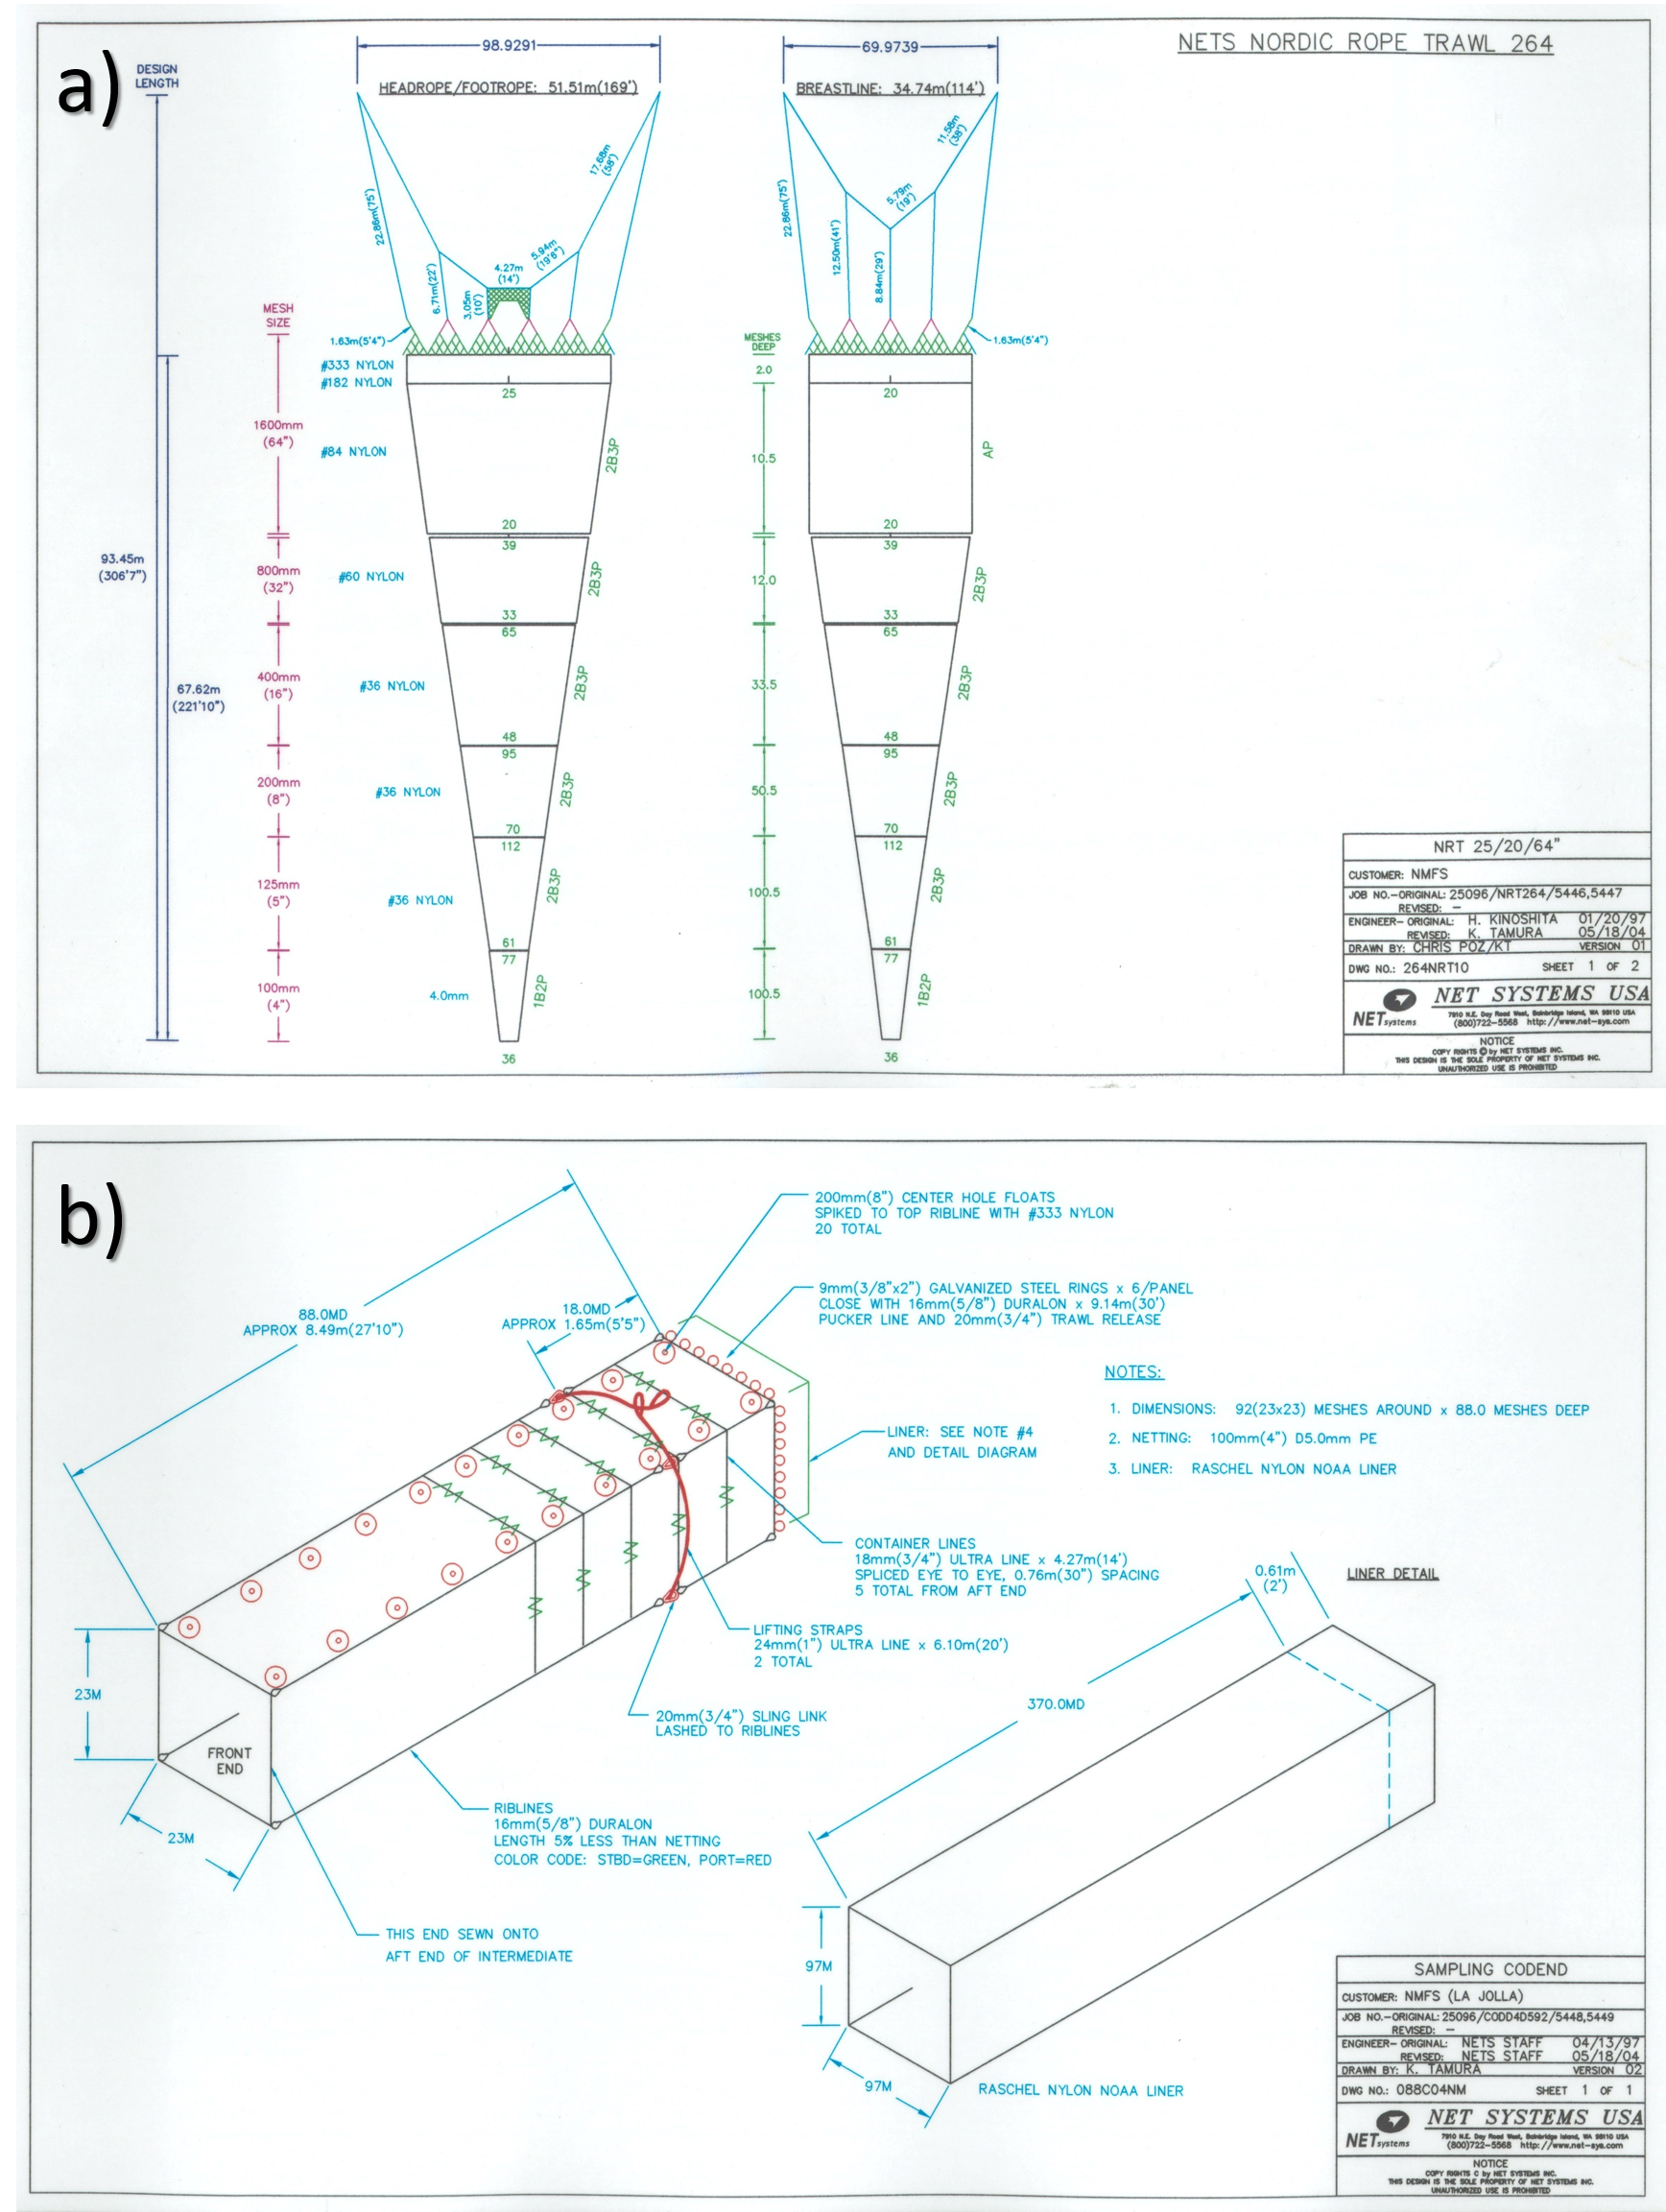
\includegraphics[width=24.11in,height=8in]{C:/CODE/estimATM/1907RL/Images/img_Nordic_264} 

}

\caption{Schematic drawings of the a) net body and b) codend of the Nordic 264 rope trawl.}\label{fig:trawl-diagrams}
\end{figure}

\newpage

\hypertarget{methods-trawl-locations}{%
\paragraph{Sampling locations}\label{methods-trawl-locations}}

Up to three nighttime (i.e., 30 min after sunset to 30 min before sunrise) surface trawls, typically spaced 10-nmi apart, were conducted in areas where echoes from putative CPS schools were observed earlier that day (\textbf{Fig. \ref{fig:trawling-locs}}). Each evening, trawl locations were selected by an acoustician who monitored CPS echoes and a member of the trawl group who measured the densities of CPS eggs in the CUFES. The locations were provided to the watch Officers who charted the proposed trawl sites.

Trawl locations were selected using the following criteria, in descending priority: CPS schools in echograms that day; CPS eggs in CUFES that day; and the trawl locations and catches during the previous night. If no CPS echoes or CPS eggs were observed along a transect that day, the trawls were alternatively placed nearshore one night and offshore the next night, with consideration given to the seabed depth and the modeled distribution of CPS habitat. Each morning, after the last trawl or 30 min prior to sunrise, \emph{Lasker} resumed sampling at the location where the acoustic sampling stopped the previous day.



\begin{figure}[H]

{\centering \includegraphics[width=3in]{C:/CODE/estimATM/1907RL/Images/img_trawl_sampling} 

}

\caption{Example of trawl paths (bold, black lines) relative to 38-kHz integrated backscattering coefficients (\(s_A\), m\textsuperscript{2} nmi\textsuperscript{-2}; averaged over 2000-m distance intervals and from 5 to 70 m deep) from putative CPS schools (colored points).}\label{fig:trawling-locs}
\end{figure}

\hypertarget{methods-trawl-processing}{%
\paragraph{Sample processing}\label{methods-trawl-processing}}

If the total volume of the trawl catch was five 35-l baskets (\textasciitilde175 l) or less, all target species were separated from the catch, sorted by species, weighed, and enumerated. If the volume of the entire catch was more than five baskets, a five-basket random subsample that included non-target species was collected, sorted by species, weighed, and enumerated; the remainder of the total catch was weighed. In these cases, the weight of the entire catch was calculated as the sum of the subsample and remainder weights. The weight of the \(e\)-th species in the total catch (\(C_{T,e}\)) was obtained by summing the catch weight of the respective species in the subsample (\(C_{S,e}\)) and the corresponding catch in the remainder (\(C_{R,e}\)), which was calculated as:

\begin{equation}
 C_{R,e} = C_R*P_{w,e}\text{,}
 \label{eq:remainder-catch-weight}
\end{equation}

where \(P_{w,e} = C_{S,e}/\sum_1^sC_{S,e}\), is the proportion in weight of the \(e\)-th species in the subsample. The number of specimens of the \(e\)-th species in the total catch (\(N_{T,e}\)) was estimated by:

\begin{equation}
 N_{T,e} = \frac{C_{T,e}}{\overline{w}_e}\text{,}
 \label{eq:number-specimens-catch}
\end{equation}

where \(\overline{w}_e\) is the mean weight of the \(e\)-th species in the subsample. For each of the target species with 50 specimens or less, individual measurements of length in mm (standard length, \(L_S\), for Pacific Sardine and Northern Anchovy, and fork length, \(L_F\), for Pacific Herring and Jack and Pacific Mackerels) and total weight (\(w\)) in g were recorded, and gonads were examined macroscopically to determine sex and reproductive stage. With the exception of Pacific Herring, the female gonads of a representative subsample of each target species were removed and preserved, and otoliths were collected for subsequent age determination. The same procedure was applied to a random sample of 50 specimens if the total number of specimens available was higher than 50.

\newpage

\hypertarget{methods-trawl-qaqc}{%
\paragraph{QA/QC}\label{methods-trawl-qaqc}}

At sea, trawl data were entered into a database (Microsoft Access). During and following the survey, data were further scrutinized, verified, and corrected if found to be erroneous. Missing length (\(L_{miss}\)) and weight (\(W_{miss}\)) measurements were estimated using the season-specific length-versus-weight relationships derived from catches during previous ATM surveys (unpublished data), where \(W_{miss} = \beta_0{L}^{\beta_1}\), \(L_{miss} = (W/\beta_0)^{(1/\beta_1)}\), and values for \(\beta_0\) and \(\beta_1\) in \textbf{Table \ref{tab:lw-conversions}}. To identify measurement or data-entry errors, length and weight data were graphically compared (\textbf{Fig. \ref{fig:lw-plot}}) to measurements from previous surveys and models of season-specific length-versus-weight from previous surveys (unpublished data). Outliers and missing values were flagged, reviewed by the trawl team, and mitigated. Catch data from aborted or otherwise unacceptable trawl hauls were removed.



\begin{table}[!h]

\caption{\label{tab:lw-conversions}General linear model (GLM) coefficients describing the total length (\(L_T\), mm) versus weight (\(W\), g) relationships used to estimate missing lengths or weights, where: \(L_T = (W/\beta_0)^{(1/\beta_1)}\) and \(W = \beta_0 {L_T}^{\beta_1}\).}
\centering
\begin{tabular}{l>{\em}lrr}
\toprule
\multicolumn{1}{c}{Common name} & \multicolumn{1}{c}{Scientific name} & \multicolumn{1}{c}{$\beta_0$} & \multicolumn{1}{c}{$\beta_1$}\\
\midrule
Pacific Herring & Clupea pallasii & 1.965e-06 & 3.253318\\
Northern Anchovy & Engraulis mordax & 2.873e-06 & 3.167299\\
Pacific Sardine & Sardinops sagax & 4.551e-06 & 3.120841\\
Pacific Mackerel & Scomber japonicus & 3.550e-06 & 3.165265\\
Jack Mackerel & Trachurus symmetricus & 5.936e-06 & 3.069390\\
\bottomrule
\end{tabular}
\end{table}



\begin{figure}[H]

{\centering \includegraphics[width=6in]{C:/CODE/estimATM/1907RL/Figs/fig_LW_plots} 

}

\caption{Specimen length-versus-weight from the current survey (colored points, by sex) compared to those from previous SWFSC surveys during the same season (gray points, all sexes). The dashed line represents the modeled length-versus-weight relationships for each species (unpublished data). Larger points indicate specimens whose length (red) or weight (blue) was missing and was estimated from the length-versus-weight relationships in \textbf{Table \ref{tab:lw-conversions}}.}\label{fig:lw-plot}
\end{figure}

\newpage

\hypertarget{methods-data-processing}{%
\subsection{Data processing}\label{methods-data-processing}}

\hypertarget{methods-acoustic-processing}{%
\subsubsection{Acoustic and oceanographic data}\label{methods-acoustic-processing}}

The calibrated echosounder data from each transect were processed using commercial software (\href{https://www.echoview.com/}{Echoview} v10.0, Echoview Software Pty Ltd.) and estimates of the sound speed and absorption coefficient calculated with contemporaneous data from CTD probes cast while stationary or underway (UCTD, see \textbf{Section \ref{methods-ctd-sampling}}). Data collected along the daytime transects at speeds \(\geq\) 5 kn were used to estimate CPS densities. Nighttime acoustic data were assumed to be negatively biased due to diel-vertical migration (DVM) and disaggregation of the target species' schools (Cutter and Demer, 2008).

\hypertarget{methods-sound-calcs}{%
\subsubsection{Sound speed and absorption calculation}\label{methods-sound-calcs}}

Depth derived from pressure in CTD casts was used to bin samples into 1-m depth increments. Sound speed in each increment (\(c_{w,i}\), m s\textsuperscript{-1}) was estimated from the average salinity, density, and pH (if measured, else pH = 8; Chen and Millero, 1977; Seabird, 2013). The harmonic sound speed in the water column (\(\overline{c}_w\), m s\textsuperscript{-1}) was calculated over the upper 70 m as:

\begin{equation}
 \overline{c}_w = \frac{\sum_{i=1}^{N} \Delta r_i}{\sum_{i=1}^{N} \Delta r_i/c_{w,i}}\text{,}
 \label{eq:time-avg-sound-speed}
\end{equation}

where \(\Delta r\) is the depth of increment \(i\) (Seabird, 2013). Measurements of seawater temperature (\(t_w\), \(^{\circ}\textrm{C}\)), salinity (\(s_w\), psu), depth, pH, and \(\overline{c}_w\) are also used to calculate the mean species-specific absorption coefficients (\(\overline{\alpha}_a\), dB m\textsuperscript{-1}) over the entire profile using equations in Francois and Garrison (1982), Ainslie and McColm (1998), and Doonan et al.~(2003). Both \(\overline{c}_w\) and \(\overline{\alpha}_a\) are later used to estimate ranges to the sound scatterers to compensate the echo signal for spherical spreading and attenuation during propagation of the sound pulse from the transducer to the scatterer range and back (Simmonds and MacLennan, 2005). The CTD rosette, when cast, also provides measures of fluorescence and dissolved oxygen concentration versus depth, which may be used to estimate the vertical dimension of Pacific Sardine potential habitat (Zwolinski \emph{et al.}, 2011), particularly the depth of the upper-mixed layer where most epipelagic CPS reside. The latter information is used to inform echo classification (see \textbf{Section \ref{methods-echo-classification}}).

\hypertarget{methods-echo-classification}{%
\subsubsection{Echo-classification}\label{methods-echo-classification}}

Echoes from schooling CPS were identified using a semi-automated data processing algorithm implemented using Echoview software (v10.0). The filters and thresholds were based on a subsample of echoes from randomly selected CPS schools. The aim of the filter criteria is to retain at least 95\% of the noise-free backscatter from CPS schools while rejecting at least 95\% of the non-CPS backscatter (\textbf{Fig. \ref{fig:ev-filtering-example}}). The filter includes the following steps:

\begin{itemize}
\tightlist
\item
  Estimate and subtract background noise using the built-in Echoview background noise removal function (De Robertis and Higginbottom, 2007, \textbf{Fig. \ref{fig:ev-filtering-example}b,e});
\item
  Average the noise-free \(S_V\) echograms using non-overlapping 11-sample by 3-ping windows;
\item
  Expand the averaged, noise-reduced \(S_V\) echograms with a 7 pixel x 7 pixel dilation;
\item
  For each pixel, compute: \(S_{V,\mathrm{200kHz}}\) - \(S_{V,\mathrm{38kHz}}\), \(S_{V,\mathrm{120kHz}}\) - \(S_{V,\mathrm{38kHz}}\), and \(S_{V,\mathrm{70kHz}}\) - \(S_{V,\mathrm{38kHz}}\);
\item
  Create a Boolean echogram for \(S_V\) differences in the CPS range: -13.85 \textless{} \(S_{V,\mathrm{70kHz}}\) - \(S_{V,\mathrm{38kHz}}\) \textless{} 9.89 \(\bigcap\) -135.5 \textless{} \(S_{V,\mathrm{120kHz}}\) - \(S_{V,\mathrm{38kHz}}\) \textless{} 9.37 \(\bigcap\) -13.51 \textless{} \(S_{V,\mathrm{200kHz}}\) - \(S_{V,\mathrm{38kHz}}\) \textless{} 12.53;
\item
  Compute the standard deviation (SD) of \(S_{V,\mathrm{120kHz}}\) and \(S_{V,\mathrm{200kHz}}\) using non-overlapping 11-sample by 3-ping windows;
\item
  Expand the SD(\(S_{V,\mathrm{120kHz}}\)) and SD(\(S_{V,\mathrm{200kHz}}\)) echograms with a 7 pixel x 7 pixel dilation;
\item
  Create a Boolean echogram based on the SDs in the CPS range: SD(\(S_{V,\mathrm{200kHz}}\)) \textgreater{} -65 dB \(\bigcap\) SD(\(S_{V,\mathrm{120kHz}}\)) \textgreater{} -65 dB. Diffuse backscattering layers (Zwolinski \emph{et al.}, 2010) have low standard deviations, whereas fish schools have high standard deviations (Demer \emph{et al.}, 2009);
\item
  Intersect the two Boolean echograms. The resulting echogram has samples with ``TRUE'' for candidate CPS schools and ``FALSE'' elsewhere;
\item
  Mask the noise-reduced echograms using the CPS Boolean echogram (\textbf{Fig. \ref{fig:ev-filtering-example}c,f});
\item
  Create an integration-start line at a range of 3 m from the transducer (\textasciitilde10 m depth);
\item
  Create an integration-stop line 3 m above the seabed (Demer \emph{et al.}, 2009), or to the maximum logging range (e.g., 350 m), whichever is shallowest;
\item
  Set the minimum \(S_V\) threshold to -60 dB (corresponding to a density of approximately three fish per 100 m\textsuperscript{3} in the case of 20-cm-long Pacific Sardine);
\item
  Integrate the volume backscattering coefficients (\(s_V\), m\textsuperscript{2} m\textsuperscript{-3}) attributed to CPS over 5-m depths and averaged over 100-m distances;
\item
  Remove regions where vessel speed was \(\leq\) 5 kn (i.e., ``on station''); and
\item
  Output the resulting nautical area scattering coefficients (\(s_A\); m\textsuperscript{2} nmi\textsuperscript{-2}) and associated information from each transect and frequency to comma-delimited text (.csv) files.
\end{itemize}

When necessary, the start and stop integration lines were manually edited to exclude reverberation due to bubbles, for the purposes of including the entirety of shallow CPS aggregations, or excluding seabed echoes.

\hypertarget{methods-backscatter-removal}{%
\subsubsection{Removal of non-CPS backscatter}\label{methods-backscatter-removal}}

In addition to echoes from target CPS, echoes may also be present from other CPS (Pacific Saury, \emph{Cololabis saira}), or semi-demersal fish such as Pacific Hake and rockfishes (\(Sebastes\) spp.). When analyzing the acoustic-survey data, it was therefore necessary to filter ``acoustic by-catch,'' i.e., backscatter not from the target species. To exclude echoes from mid-water, demersal, and benthic fishes, vertical temperature profiles were superimposed on the echo-integrated data for each transect. Echoes below the surface mixed layer were excluded from the CPS analysis (\textbf{Fig. \ref{fig:ctd-app}}). In areas dominated by Pacific Herring, for example off Vancouver Island, backscatter was integrated to a maximum depth of 75 m.



\begin{figure}[H]

{\centering \includegraphics[width=6.5in]{C:/CODE/estimATM/1907RL/Images/img_echoview_filtering_example-labeled} 

}

\caption{Echogram depicting CPS schools (red) and plankton aggregations (blue and green) at 38 kHz (top) and 120 kHz (bottom). Example data processing steps include the original echogram (left), after noise subtraction and bin-averaging (middle), and filtering to retain only putative CPS echoes (right).}\label{fig:ev-filtering-example}
\end{figure}

\newpage



\begin{figure}[H]

{\centering \includegraphics[width=5.5in]{C:/CODE/estimATM/1907RL/Images/img_ctd_app} 

}

\caption{Temperature profiles (left) and the distribution of echoes from fishes with swimbladders (blue points, scaled by backscatter intensity; right) along an example acoustic transect. In this example, temperature profiles indicate an \textasciitilde25 m-deep mixed-layer above an \textasciitilde20-30 m thermocline, so the 11 \(^{\circ}\textrm{C}\) isotherm (bold, blue line; right panel) was used to remove echoes from deeper, bottom-dwelling schools of non-CPS fishes with swimbladders. The proximity of the echoes to the seabed (bold, red line; right panel) was also used to define the lower limit for vertical integration.}\label{fig:ctd-app}
\end{figure}

\hypertarget{methods-acoustics-qaqc}{%
\subsubsection{QA/QC}\label{methods-acoustics-qaqc}}

The largest 38-kHz integrated backscattering coefficient values (\(s_A\), m\textsuperscript{2} nmi\textsuperscript{-2}) were graphically examined to identify potential errors in the integrated data from Echoview processing (e.g., when a portion of the seabed was accidentally integrated, \textbf{Fig. \ref{fig:nasc-outliers}}). If found, errors were corrected and data were re-integrated prior to use for biomass estimation.



\begin{figure}[H]

{\centering \includegraphics[width=4.15in]{C:/CODE/estimATM/1907RL/Figs/fig_nasc_outliers} 

}

\caption{Ranked 38-kHz integrated backscattering coefficient values (\(s_A\), m\textsuperscript{2} nmi\textsuperscript{-2}; n = 100), labeled with the vessel name (\(RL\) = \emph{Lasker}, SD1024 = Saildrone USV), transect number, and echogram distance interval. The \(s_A\) values for the 100-m intervals are divided by 19 for scaling to the traditional horizontal bin length, or Elementary Distance Sampling Unit (EDSU), of 1 nmi.}\label{fig:nasc-outliers}
\end{figure}



\hypertarget{methods-echointegration}{%
\subsubsection{Echo integral partitioning and acoustic inversion}\label{methods-echointegration}}

For fishes with swimbladders, the acoustic backscattering cross-section of an individual (\(\sigma_{bs}\), m\textsuperscript{2}) depends on many factors but mostly on the acoustic wavelength and the swimbladder size and orientation relative to the incident sound pulse. For echosounder sampling conducted in this survey, \(\sigma_{bs}\) is a function of the dorsal-surface area of the swimbladder and was approximated by a function of fish length, i.e.:

\begin{equation}
  \sigma_{bs} = 10^{\frac{m\,\log_{10}(L)+b}{10}}\text{,}
  \label{eq:sigma-bs}
\end{equation}

where \(m\) and \(b\) are frequency and species-specific parameters that are obtained theoretically or experimentally (see references below). \(TS\), a logarithmic representation of \(\sigma_{bs}\), is defined as:

\begin{equation}
  TS = 10\,\log_{10}(\sigma_{bs}) = m\,\log_{10}(L) + b\text{.}
  \label{eq:ts-sigma-bs-equation}
\end{equation}

\(TS\) has units of dB re 1 m\textsuperscript{2} if defined for an individual, or dB re 1 m\textsuperscript{2} kg\textsuperscript{-1} if defined by weight. The following equations for \(TS_{38\mathrm{kHz}}\) were used in this analysis:

\begin{equation}
  TS_{\mathrm{38kHz}} = -14.90 \times (\log_{10} (L_T) - 13.21 \text{, for Pacific Sardine;}
  \label{eq:tl-ts-sardine}
\end{equation}

\begin{equation}
  TS_{\mathrm{38kHz}} = -11.97 \times (\log_{10} (L_T) - 11.58561 \text{, for Pacific Herring;}
  \label{eq:tl-ts-herring}
\end{equation}

\begin{equation}
  TS_{\mathrm{38kHz}} = -13.87 \times (\log_{10} (L_T) - 11.797 \text{, for Northern Anchovy; and}
  \label{eq:tl-ts-anchovy}
\end{equation}

\begin{equation}
  TS_{\mathrm{38kHz}} = -15.44 \times (\log_{10} (L_T) - 7.75 \text{, for Pacific and Jack Mackerels,}
  \label{eq:tl-ts-mackerel}
\end{equation}

where the units for total length (\(L_T\)) is cm and \(TS\) is dB re 1 m\textsuperscript{2} kg\textsuperscript{-1}.

Equations \eqref{eq:tl-ts-sardine} and \eqref{eq:tl-ts-mackerel} were derived from echosounder measurements of in situ \(\sigma_{bs}\) and measures of \(L_T\) and \(W\) from concomitant catches of South American Pilchard (\emph{Sardinops ocellatus}) and Horse Mackerel (\emph{Trachurus trachurus}) off South Africa (Barange \emph{et al.}, 1996). Because mackerels have similar \(TS\) (Peña, 2008), Equation \eqref{eq:tl-ts-mackerel} is used for Pacific and Jack Mackerels. For Pacific Herring, Equation \eqref{eq:tl-ts-herring} was derived from that of Thomas et al.~(2002) measured at 120 kHz with the following modifications: 1) the intercept used here was calculated as the average intercept of Thomas et al.'s spring and fall regressions; 2) the intercept was compensated for swimbladder compression after Zhao et al.~(2008) using the average depth for Pacific Herring of 44 m; 3) the intercept was increased by 2.98 dB to account for the change of frequency from 120 to 38 kHz (Saunders \emph{et al.}, 2012). For Northern Anchovy, Equation \eqref{eq:tl-ts-anchovy} was derived from that of Kang et al.~(2009), after compensation of the swimbladder volume (Ona, 2003; Zhao \emph{et al.}, 2008) for the average depth of Northern Anchovy observed in summer 2016 (19 m, Zwolinski \emph{et al.}, 2017).

To calculate \(TS_{38\mathrm{kHz}}\), \(L_T\) (cm) was estimated from measurements of standard length (\(L_S\)) or fork length (\(L_F\); cm) using linear relationships between length and weight derived from specimens collected in the CCE: for Pacific Sardine, \(L_T = 0.3574 + 1.149L_S\); for Northern Anchovy, \(L_T = 0.2056 + 1.1646 L_S\); for Pacific Mackerel, \(L_T = 0.2994 + 1.092 L_F\); for Jack Mackerel \(L_T = 0.7295 + 1.078 L_F\); and for Pacific Herring \(L_T = -0.105 + 1.2 L_F\).



The proportions of species in a trawl cluster were considered representative of the proportions of species in the vicinity of the cluster. Therefore, the proportion of the echo-integral from the \(e\)-th species (\(P_e\)) in an ensemble of \(s\) species can be calculated from the species catches \(N_1, N_2,..., N_s\) and the respective average backscattering cross-sections \(\sigma_{bs_1}, \sigma_{bs_2},...,\sigma_{bs_s}\) (Nakken and Dommasnes, 1975). The acoustic proportion for the \(e\)-th species in the \(a\)-th trawl (\(P_{ae}\)) is:

\begin{equation}
 P_{ae} = \frac{N_{ae} \times \overline{w}_{ae} \times \overline{\sigma}_{bs,ae}}{\sum_{e=1}^{s_a} (N_{ae} \times \overline{w}_{ae} \times \overline{\sigma}_{bs,ae})}\text{, }
  \label{eq:acoustic-prop-spp}
\end{equation}

where \(\overline{\sigma}_{bs,ae}\) is the arithmetic counterpart of the average target strength (\(\overline{TS}_{ae}\)) averaged for all \(n_{ae}\) individuals of species \(e\) in the random sample of trawl \(a\):

\begin{equation}
  \overline{\sigma}_{bs,ae} = \frac{\sum_{i=1}^{n_{ae}}10^{(TS_i/10)}}{n_{ae}}\text{, }
  \label{eq:avg-ts-all-spp}
\end{equation}

and \(\overline{w}_{ae}\) is the average weight: \(\overline{w}_{ae} = \sum_{i=1}^{n_{ae}}{w_{aei}}/{n_{ae}}\). The total number of individuals of species \(e\) in a trawl \(a\) (\(N_{ae}\)) is obtained by: \(N_{ae}=\frac{n_{ae}}{w_{s,ae}} \times w_{t,ae}\), where \(w_{s,ae}\) is the weight of the \(n_{ae}\) individuals sampled randomly, and \(w_{t,ae}\) is the total weight of the respective species' catch.

The trawls within a cluster were combined to reduce sampling variability (see \textbf{Section \ref{methods-trawl-clustering}}), and the number of individuals caught from the \(e\)-th species in a cluster \(g\) (\(N_{ge}\)) was obtained by summing the catches across the \(h\) trawls in the cluster: \(N_{ge}=\sum_{a=1}^{h_g}N_{ae}\). The backscattering cross-section for species \(e\) in the \(g\)-th cluster with \(a\) trawls is then given by:

\begin{equation}
  \overline{\sigma}_{bs,ge}=\frac{\sum_{a=1}^{h_g} N_{ae} \times \overline{w}_{ae} \times \overline{\sigma}_{bs,ae}}{\sum_{a=1}^{s_g} N_{ae} \times \overline{w}_{ae}}\text{, }
  \label{eq:sigma-spp-j}
\end{equation}

where:

\begin{equation}
  \overline{w}_{ge} = \frac{\sum_{a=1}^{h_g} N_{ae} \times \overline{w}_{ae}}{\sum_{a=1}^{h_g} N_{ae}}\text{, }
  \label{eq:w-spp-j}
\end{equation}

and the proportion (\(P_{ge}\)) is;

\begin{equation}
  P_{ge} = \frac{N_{ge} \times \overline{w}_{ge} \times \overline{\sigma}_{bs,ae}}{\sum_{e=1}^{s}(N_{ge} \times \overline{w}_{ge} \times \overline{\sigma}_{bs,ge})}\text{.}
  \label{eq:prop-spp-j}
\end{equation}

\hypertarget{methods-trawl-clustering}{%
\subsubsection{Trawl clustering and species proportions}\label{methods-trawl-clustering}}

Trawls that occurred on the same night were assigned to a trawl cluster. Biomass densities (\(\rho\)) were calculated for 100-m transect intervals by dividing the integrated area backscatter coefficients for each CPS species by the mean backscattering cross-sectional area (MacLennan \emph{et al.}, 2002) estimated in the trawl cluster nearest in space. Survey data were post-stratified to account for spatial heterogeneity in sampling effort and biomass density in a similar way to that performed for Pacific Sardine (Zwolinski \emph{et al.}, 2016).

For a generic 100-m long acoustic interval, the area backscattering coefficient for species \(e\): \(s_{A,e} = s_{A,cps} \times P_{ge}\), where \(P_{ge}\) is the species acoustic proportion of the nearest trawl cluster (Equation \eqref{eq:prop-spp-j}), was used to estimate the biomass density (\(\rho_{w,e}\)) (MacLennan \emph{et al.}, 2002; Simmonds and MacLennan, 2005) for every 100-m interval, using the size and species composition of the nearest (space and time) trawl cluster (\textbf{Fig. \ref{fig:trawl-cluster-map}}):

\begin{equation}
  \rho_{w,e} = \frac{s_{A,e}}{4\pi\overline{\sigma}_{bs,e}}\text{.}
  \label{eq:biomass-density}
\end{equation}

The biomass densities were converted to numerical densities using: \(\rho_{n,e}=\rho_{w,e}/\overline{w}_e\), where \(\overline{w}_e\) is the corresponding mean weight. Also, for each acoustic interval, the biomass or numeric densities are partitioned into length classes according to the species' length distribution in the respective trawl cluster.

\hypertarget{removal-of-coincident-sampling}{%
\subsubsection{Removal of coincident sampling}\label{removal-of-coincident-sampling}}

To avoid overestimation of biomass in areas sampled by both vessels, USV samples were omitted within the area sampled by \emph{Lasker}.

\hypertarget{methods-data-analysis}{%
\subsection{Data analysis}\label{methods-data-analysis}}

\hypertarget{methods-post-stratification}{%
\subsubsection{Post-stratification}\label{methods-post-stratification}}

The transects were used as sampling units (Simmonds and Fryer, 1996). Because each species does not generally span the entire survey area (Demer and Zwolinski, 2017; Zwolinski \emph{et al.}, 2014), the sampling domain was stratified for each species and stock. Strata were defined by uniform transect spacing (sampling intensity) and either presences (positive densities and potentially structural zeros) or absences (real zeros) of species biomass. Each stratum has: 1) at least three transects, with approximately equal spacing, 2) fewer than three consecutive transects with zero-biomass density, and 3) bounding transects with zero-biomass density (\textbf{Figs. \ref{fig:tx-biom-dens}}, \textbf{\ref{fig:acoustic-strata-map}}). This approach tracks stock patchiness and creates statistically-independent, stationary, post-sampling strata (Johannesson and Mitson, 1983; Simmonds \emph{et al.}, 1992). For Northern Anchovy, we define the separation between the northern and central stock at Cape Mendocino (40.4 \(^{\circ}\textrm{N}\)). For Pacific Sardine, we define the separation between the northern and southern stock by the boundary between their respective potential oceanographic habitats (Demer and Zwolinski, 2014; Zwolinski \emph{et al.}, 2011), in this case at Point Conception (34.7 \(^{\circ}\textrm{N}\)).



\begin{figure}[H]

{\centering \includegraphics[width=4.5in]{C:/CODE/estimATM/1907RL/Figs/fig_nasc_cluster_trawl_proportion} 

}

\caption{a) Polygons enclosing 100-m acoustic intervals assigned to each trawl cluster, and b) the proportion (by weight) of CPS in each trawl cluster. The numbers inside each polygon in panel a) are the cluster numbers, which are located at the average latitude and longitude of all trawls in that cluster. Black points in panel b) indicate trawl clusters with no CPS present.}\label{fig:trawl-cluster-map}
\end{figure}

\newpage



\newpage
\blandscape

\begin{figure}[H]

{\centering \includegraphics[width=8.5in]{C:/CODE/estimATM/1907RL/Figs/fig_biomass_density_transect_lat} 

}

\caption{Acoustic biomass density (\(\log_{10}(t+1)\) nmi\textsuperscript{-2}) versus latitude (easternmost portion of each transect) and strata used to estimate biomass and abundance (shaded regions; outline indicates stratum number) for each species and survey vessel (labels above plots; \emph{RL} = \emph{Lasker}, SD1024 = Saildrone USV). Strata with no outline were not included because of too few specimens (\textless{} 10 individuals), trawl clusters (\textless{} 2 clusters), or both. Blue number labels correspond to transects with positive biomass (\(\log_{10}(t+1)\) \textgreater{} 0.01). Point fills indicate transect spacing (nmi). Dashed horizontal lines indicate prominent biogeographic landmarks used to delineate stock boundaries for Northern Anchovy and Pacific Sardine.}\label{fig:tx-biom-dens}
\end{figure}

\elandscape
\newpage



\begin{figure}[H]

{\centering \includegraphics[width=48.53in,height=8in]{C:/CODE/estimATM/1907RL/Figs/fig_acoustic_strata} 

}

\caption{Post-survey stratification indicating stratum polygons (outline indicates stratum number; fill indicates the species' stock designation) used to estimate the biomasses of CPS. Point sizes indicate the relative intensity (\(s_A\); m\textsuperscript{2} nmi\textsuperscript{-2}) of acoustic backscatter from all CPS (black points) and individual species (red points). Smaller nearshore strata (e.g., Northern Anchovy sampled by the USV) may be difficult to visualize at this scale.}\label{fig:acoustic-strata-map}
\end{figure}

\newpage

\hypertarget{methods-biomass-and-precision}{%
\subsubsection{Estimation of biomass and sampling precision}\label{methods-biomass-and-precision}}

For each stratum and stock, the biomass (\(B\); kg) of each species was estimated by:

\begin{equation}
  \hat{B} = A \times \hat{D}\text{, }
  \label{eq:biomass-mean}
\end{equation}

where \(A\) is the stratum area (nmi\textsuperscript{2}) and \(\hat{D}\) is the estimated mean biomass density (kg nmi\textsuperscript{-2}):

\begin{equation}
  \hat{D} = \frac{\sum_{l=1}^{k}\overline{\rho}_{w,l} c_l}{\sum_{l=1}^{k}c_l}\text{, }
  \label{eq:biomass-mean-density}
\end{equation}

where \(\overline{\rho}_{w,l}\) is the mean biomass density of the species on transect \(l\), \(c_l\) is the transect length, and \(k\) is the total number of transects. The variance of \(\hat{B}\) is a function of the variability of the transect-mean densities and associated lengths. Treating transects as replicate samples of the underlying population (Simmonds and Fryer, 1996), the variance was calculated using bootstrap resampling (Efron, 1981) based on transects as sampling units. Provided that each stratum has independent and identically-distributed transect means (i.e., densities on nearby transects are not correlated, and they share the same statistical distribution), bootstrap or other random-sampling estimators provide unbiased estimates of variance.

The 95\% confidence intervals (CI\textsubscript{95\%}) for the mean biomass densities (\(\hat{D}\)) were estimated as the 0.025 and 0.975 percentiles of the distribution of 5 bootstrap survey-mean biomass densities. Coefficient of variation (CV, \%) values were obtained by dividing the bootstrapped standard error by the mean estimate (Efron, 1981). Total biomass in the survey area was estimated as the sum of the biomasses in each stratum, and the associated sampling variance was calculated as the sum of the variances across strata.

\hypertarget{methods-abundance-at-length}{%
\subsubsection{Abundance- and biomass-at-length estimates}\label{methods-abundance-at-length}}

The numerical densities by length class (\textbf{Section \ref{methods-trawl-clustering}}) were averaged for each stratum in a similar way for that used for biomass (Equation \eqref{eq:biomass-mean-density}), and raised to the stratum area to obtain abundance per length class.

\hypertarget{methods-cluster-biomass-density}{%
\subsubsection{Percent contribution of acoustic biomass per cluster}\label{methods-cluster-biomass-density}}

The percent contribution of each cluster to the estimated abundance in a stratum (\textbf{Appendix \ref{appendix-cluster-length-percent}}) was calculated as:

\begin{equation}
  \frac{\Sigma_{i = 1}^{l}\overline{\rho}_{ci}}{\Sigma_{c=1}^{C}\Sigma_{i=1}^{l}\overline{\rho}_{ci}}{\text{,}}
  \label{eq:pct-acoustic-biomass}
\end{equation}

where \(\overline{\rho}_{ci}\) is the numerical density in interval \(i\) represented by the nearest trawl cluster \(c\).

\newpage

\hypertarget{results}{%
\section{Results}\label{results}}

\hypertarget{results-sampling-effort}{%
\subsection{Sampling effort and allocation}\label{results-sampling-effort}}

The summer 2019 survey took place between Cape Scott, Vancouver Island and San Diego during 77 DAS between 12 June and 10 September 2019. Acoustic sampling was conducted along 84 daytime east-west transects (84 by \emph{Lasker} and 0 by the USV) that totaled 3,837 nmi (3,837 nmi by \emph{Lasker} and by the USV). Catches from a total of 99 nighttime surface trawls were combined into 38 trawl clusters. As many as two post-survey strata were defined considering transect spacing and the densities of echoes attributed to CPS. Biomasses and abundances were estimated for each species.

\textbf{Leg I}\\
On 26 June, \emph{Lasker} departed from the Exploratorium (Pier 15) in San Francisco at \textasciitilde2130 (all times GMT) and began the offshore transit to northern Vancouver Island. Throughout the transit, sampling was conducted during the day with CUFES, EK60s, ME70, MS70 and SX90. The EK80 was run at night only. On 1 July, \emph{Lasker} arrived at the first nearshore station off Cape Scott at \textasciitilde1300 to begin acoustic sampling along transect 126. Acoustic sampling ceased after the completion of transect 90 off Tillamook Bay. On 16 July, \emph{Lasker} arrived at the Marine Operations-Pacific (MOC-P) Pier in Newport, OR at \textasciitilde1700 to complete Leg I.

\textbf{Leg II}\\
On 21 July, \emph{Lasker} departed from MOC-P Pier in Newport at \textasciitilde0200, and arrived at transect 90 off Tillamook Bay at \textasciitilde1240 on 21 July to resume survey operations. On 8 August, acoustic sampling ceased after the completion of transect 58 off Cape Mendocino. On 9 August, \emph{Lasker} arrived at the Exploratorium (Pier 15) in San Francisco at \textasciitilde1300 to complete Leg II.

\textbf{Leg III}\\
On 13 August, \emph{Lasker} departed from the Exploratorium (Pier 15) in San Francisco at \textasciitilde2200, and arrived at transect 58 off Cape Mendocino at \textasciitilde1750 on 14 August to resume survey operations. On 28 August, the final day of acoustic transects, transect 29 was not completed before sunset, and needed to be resampled during Leg IV. On 29 August, at the end of the offshore marine mammal line, a planned trawl was not feasible due to a chaffed line that required repair. On 31 August, \emph{Lasker} arrived at the 10th Avenue Marine Terminal in San Diego to complete Leg III.

\textbf{Leg IV}\\
On 5 September, \emph{Lasker} departed from the fuel dock of 10th Avenue Marine Terminal in San Diego at \textasciitilde2345. At \textasciitilde0200 on 7 September, \emph{Lasker} resumed survey operations at the first station south of Big Sur, near the nearshore segment of transects 28/29. On 23 September, survey operations concluded with \emph{Lasker}'s arrival to the 10th Avenue Marine Terminal in San Diego at 0230.

On NA, the USV (SD-1024) departed San Francisco and sampled southward. On NA, the USV ceased sampling off Pt. Conception and returned to San Francisco.

\hypertarget{results-backscatter-distribution}{%
\subsection{Acoustic backscatter}\label{results-backscatter-distribution}}

The majority of acoustic backscatter ascribed to CPS was observed near Cape Flattery; between Westport and Cape Mendocino; and between San Francisco and San Diego (\textbf{Fig. \ref{fig:nasc-cufes-trawl}a}). Some acoustic backscatter ascribed to CPS was also observed by the USV nearshore between San Francisco and Morro Bay (\textbf{Fig. \ref{fig:nasc-saildrone}}). The majority (\textasciitilde90\%) of acoustic biomass for each species was apportioned using catch data from trawl clusters conducted within a distance of \(\leq\) 30 nmi (\textbf{Fig. \ref{fig:biomass-cluster-distance}}).

\hypertarget{results-cufes-density}{%
\subsection{Egg densities and distributions}\label{results-cufes-density}}

Northern Anchovy eggs were most abundant in the CUFES samples nearshore between Westport and Tillamook in the north, and between San Francisco and Morro Bay in central CA (\textbf{Fig. \ref{fig:nasc-cufes-trawl}b}). Jack Mackerel eggs were observed offshore from central Vancouver Island to Tillamook, between San Francisco and Big Sur, and to a lesser extent between Cape Blanco and Fort Bragg (\textbf{Fig. \ref{fig:nasc-cufes-trawl}b}). Pacific Sardine eggs observed in the CUFES samples were most abundant offshore of Tillamook (\textbf{Fig. \ref{fig:nasc-cufes-trawl}b}, obscured by Northern Anchovy and Jack Mackerel eggs); some Pacific Sardine eggs were present in CUFES samples offshore between Cape Mendocino and San Francisco, near San Miguel Island, and near San Diego (\textbf{Fig. \ref{fig:nasc-cufes-trawl}b}). There was little overlap in the distribution of Northern Anchovy, Pacific Sardine, and Jack Mackerel eggs in CUFES samples. The concentrations of Northern Anchovy eggs in the CUFES samples were coincident with CPS backscatter.

\hypertarget{results-trawl-catch}{%
\subsection{Trawl catch}\label{results-trawl-catch}}

Jack Mackerel comprised the greatest proportion of catch in trawl samples between the Columbia River and San Francisco (\textbf{Fig. \ref{fig:nasc-cufes-trawl}c}). Pacific Herring comprised the greatest proportion of catch in trawl samples nearshore along the coast of Vancouver Island and around Newport (\textbf{Fig. \ref{fig:nasc-cufes-trawl}c}). Northern Anchovy were predominantly found in trawls conducted between San Francisco and San Diego, with some present between Westport and the Columbia River (\textbf{Fig. \ref{fig:nasc-cufes-trawl}c}). Pacific Sardine were collected in trawls conducted between Newport and Coos Bay, and between Point Conception and Long Beach, CA. Overall, the 99 trawls captured a combined 8,073 kg of CPS (0 kg of Northern Anchovy, 0 kg of Pacific Sardine, 0 kg of Pacific Mackerel, 0 kg of Jack Mackerel, and 0 kg Pacific Herring).

\newpage  
\blandscape



\begin{figure}[H]

{\centering \includegraphics[width=8.5in]{C:/CODE/estimATM/1907RL/Figs/fig_nasc_cufes_trawl_proportion} 

}

\caption{Spatial distributions of: a) 38-kHz integrated backscattering coefficients (\(s_A\), m\textsuperscript{2} nmi\textsuperscript{-2}; averaged over 2000-m distance intervals and from 5 to 70 m deep) ascribed to CPS; b) CUFES egg density (eggs m\textsuperscript{-3}) for Northern Anchovy, Pacific Sardine, and Jack Mackerel; and c) acoustic proportions of CPS in trawl clusters (black points indicate trawl clusters with no CPS).}\label{fig:nasc-cufes-trawl}
\end{figure}

\elandscape
\newpage



\newpage
\blandscape



\begin{figure}[H]

{\centering \includegraphics[width=9in]{C:/CODE/estimATM/1907RL/Figs/fig_cluster_distance_cumulative_biomass} 

}

\caption{Total (top) and cumulative (bottom) acoustic biomass (t) versus distance to the nearest positive trawl cluster.}\label{fig:biomass-cluster-distance}
\end{figure}

\elandscape  
\newpage

\hypertarget{results-biomass-distribution}{%
\subsection{Biomass distribution and demography}\label{results-biomass-distribution}}

\hypertarget{results-anchovy}{%
\subsubsection{Northern Anchovy}\label{results-anchovy}}

\hypertarget{results-anchovy-northern} = 690 - 2,337 t, CV = 53\%; \textbf{Table \ref{tab:biomass-anch-n}}). The northern stock ranged from approximately Westport, WA to Coos Bay, OR (\textbf{Fig. \ref{fig:biom-dens-anch-n}}). The \(L_S\) ranged from 12 to 18 cm with a mode at \textasciitilde13 cm (\textbf{Table \ref{tab:l-freq-summ-anch-n}}, \textbf{Fig. \ref{fig:l-disagg-anch-n}}).



\begin{table}[!h]

\caption{\label{tab:biomass-anch-n}Biomass estimates (metric tons, t) and their precision (upper and lower 95\% confidence intervals, CI\textsubscript{95\%}; standard deviation, SD; and coefficient of variation, CV) for the northern stock of Northern Anchovy (\emph{Engraulis mordax}). Stratum areas are nmi\textsuperscript{2}.}
\centering
\resizebox{\linewidth}{!}{
\fontsize{8}{10}\selectfont
\begin{tabular}{>{\em}l|c|r|r|r|r|r|r|r|r|r|r}
\hline
\multicolumn{2}{c|}{Species} & \multicolumn{4}{c|}{Stratum} & \multicolumn{2}{c|}{Trawl} & \multicolumn{4}{c}{Biomass} \\
\cline{1-2} \cline{3-6} \cline{7-8} \cline{9-12}
Name & Stock & Number & Area & Transects & Distance & Clusters & Individuals & Mean & CI$_{L,95\%}$ & CI$_{U,95\%}$ & CV\\
\hline
\rowcolor{gray!6}   &  & 2 & 11,589 & 22 & 1,159 & 6 & 904 & 1,515 & 690 & 2,337 & 53\\
\cline{3-12}
\multirow{-2}{*}{\raggedright\arraybackslash Engraulis mordax} & \multirow{-2}{*}{\centering\arraybackslash Northern} & All & 11,589 & 22 & 1,159 & 6 & 904 & 1,515 & 690 & 2,337 & 53\\
\hline
\end{tabular}}
\end{table}

\hypertarget{results-anchovy-central} = 60,042 - 109,867 t, CV = 26\%; \textbf{Table \ref{tab:biomass-anch-c}}). The central stock ranged from approximately Bodega Bay to San Diego, CA (\textbf{Fig. \ref{fig:biom-dens-anch-c}}). \(L_S\) ranged from 10 to 16 cm with modes at 10 and 12 cm (\textbf{Table \ref{tab:l-freq-summ-anch-c}}, \textbf{Fig. \ref{fig:l-disagg-anch-c}}). USV sampling nearshore (stratum 5) added t or \textasciitilde\% to the biomass sampled offshore (88,878.5 t).



\begin{table}[!h]

\caption{\label{tab:biomass-anch-c}Biomass estimates (metric tons, t) and their precision (upper and lower 95\% confidence intervals, CI\textsubscript{95\%}; standard deviation, SD; and coefficient of variation, CV) for the central stock of Northern Anchovy (\emph{Engraulis mordax}). Stratum areas are nmi\textsuperscript{2}.}
\centering
\resizebox{\linewidth}{!}{
\fontsize{8}{10}\selectfont
\begin{tabular}{>{\em}l|c|r|r|r|r|r|r|r|r|r|r}
\hline
\multicolumn{2}{c|}{Species} & \multicolumn{4}{c|}{Stratum} & \multicolumn{2}{c|}{Trawl} & \multicolumn{4}{c}{Biomass} \\
\cline{1-2} \cline{3-6} \cline{7-8} \cline{9-12}
Name & Stock & Number & Area & Transects & Distance & Clusters & Individuals & Mean & CI$_{L,95\%}$ & CI$_{U,95\%}$ & CV\\
\hline
\rowcolor{gray!6}   &  & 1 & 6,198 & 16 & 634 & 4 & 60,049 & 88,879 & 60,042 & 109,867 & 26\\
\cline{3-12}
\multirow{-2}{*}{\raggedright\arraybackslash Engraulis mordax} & \multirow{-2}{*}{\centering\arraybackslash Central} & All & 6,198 & 16 & 634 & 4 & 60,049 & 88,879 & 60,042 & 109,867 & 26\\
\hline
\end{tabular}}
\end{table}

\newpage



\begin{longtable}{>{\em}l|l|r|r}
\caption{\label{tab:l-freq-summ-anch-n}Abundance versus standard length (\(L_S\), cm) for the northern stock of Northern Anchovy (\emph{Engraulis mordax}).}\\
\hline
\multicolumn{1}{c}{Species} & \multicolumn{1}{c}{Stock} & \multicolumn{1}{c}{$L_S$} & \multicolumn{1}{c}{Abundance}\\
\hline
\rowcolor{gray!6}   &  & 1 & 0\\
\cline{3-4}
 &  & 2 & 0\\
\cline{3-4}
\rowcolor{gray!6}   &  & 3 & 0\\
\cline{3-4}
 &  & 4 & 0\\
\cline{3-4}
\rowcolor{gray!6}   &  & 5 & 0\\
\cline{3-4}
 &  & 6 & 0\\
\cline{3-4}
\rowcolor{gray!6}   &  & 7 & 0\\
\cline{3-4}
 &  & 8 & 0\\
\cline{3-4}
\rowcolor{gray!6}   &  & 9 & 0\\
\cline{3-4}
 &  & 10 & 0\\
\cline{3-4}
\rowcolor{gray!6}   &  & 11 & 0\\
\cline{3-4}
 &  & 12 & 49,283\\
\cline{3-4}
\rowcolor{gray!6}   &  & 13 & 299,629\\
\cline{3-4}
 &  & 14 & 2,546,341\\
\cline{3-4}
\rowcolor{gray!6}   &  & 15 & 9,747,972\\
\cline{3-4}
 &  & 16 & 5,752,151\\
\cline{3-4}
\rowcolor{gray!6}   &  & 17 & 10,373,984\\
\cline{3-4}
 &  & 18 & 2,522,156\\
\cline{3-4}
\rowcolor{gray!6}   &  & 19 & 0\\
\cline{3-4}
\multirow{-20}{*}{\raggedright\arraybackslash Engraulis mordax} & \multirow{-20}{*}{\raggedright\arraybackslash Northern} & 20 & 0\\
\hline
\end{longtable}



\begin{longtable}{>{\em}l|l|r|r}
\caption{\label{tab:l-freq-summ-anch-c}Abundance versus standard length (\(L_S\), cm) for the central stock of Northern Anchovy (\emph{Engraulis mordax}).}\\
\hline
\multicolumn{1}{c}{Species} & \multicolumn{1}{c}{Stock} & \multicolumn{1}{c}{$L_S$} & \multicolumn{1}{c}{Abundance}\\
\hline
\rowcolor{gray!6}   &  & 1 & 0\\
\cline{3-4}
 &  & 2 & 0\\
\cline{3-4}
\rowcolor{gray!6}   &  & 3 & 0\\
\cline{3-4}
 &  & 4 & 0\\
\cline{3-4}
\rowcolor{gray!6}   &  & 5 & 0\\
\cline{3-4}
 &  & 6 & 0\\
\cline{3-4}
\rowcolor{gray!6}   &  & 7 & 0\\
\cline{3-4}
 &  & 8 & 0\\
\cline{3-4}
\rowcolor{gray!6}   &  & 9 & 0\\
\cline{3-4}
 &  & 10 & 79,209,121\\
\cline{3-4}
\rowcolor{gray!6}   &  & 11 & 581,794,465\\
\cline{3-4}
 &  & 12 & 587,192,836\\
\cline{3-4}
\rowcolor{gray!6}   &  & 13 & 1,326,227,317\\
\cline{3-4}
 &  & 14 & 1,031,520,943\\
\cline{3-4}
\rowcolor{gray!6}   &  & 15 & 143,309,866\\
\cline{3-4}
 &  & 16 & 7,528,339\\
\cline{3-4}
\rowcolor{gray!6}   &  & 17 & 0\\
\cline{3-4}
 &  & 18 & 0\\
\cline{3-4}
\rowcolor{gray!6}   &  & 19 & 0\\
\cline{3-4}
\multirow{-20}{*}{\raggedright\arraybackslash Engraulis mordax} & \multirow{-20}{*}{\raggedright\arraybackslash Central} & 20 & 0\\
\hline
\end{longtable}

\newpage



\begin{figure}[H]

{\centering \includegraphics[width=18.65in,height=8.35in]{C:/CODE/estimATM/1907RL/Figs/fig_biomass_dens_map_Engraulis mordax-Northern} 

}

\caption{Biomass densities of northern stock of Northern Anchovy (\emph{Engraulis mordax}), per strata, throughout the survey region. The blue numbers represent the locations of trawl clusters with at least one anchovy. The gray line represents the vessel track.}\label{fig:biom-dens-anch-n}
\end{figure}

\newpage



\begin{figure}[H]

{\centering \includegraphics[width=25in,height=6in]{C:/CODE/estimATM/1907RL/Figs/fig_L_disagg_Engraulis mordax-Northern} 

}

\caption{Abundance versus standard length (\(L_S\), upper panel) and biomass (t) versus \(L_S\) (lower panel) for the northern stock of Northern Anchovy (\emph{Engraulis mordax}) in the survey area.}\label{fig:l-disagg-anch-n}
\end{figure}

\newpage



\begin{figure}[H]

{\centering \includegraphics[width=18.65in,height=8.35in]{C:/CODE/estimATM/1907RL/Figs/fig_biomass_dens_map_Engraulis mordax-Central} 

}

\caption{Biomass densities of central stock of Northern Anchovy (\emph{Engraulis mordax}), per strata, throughout the survey region. The blue numbers represent the locations of trawl clusters with at least one anchovy. The gray line represents the vessel track.}\label{fig:biom-dens-anch-c}
\end{figure}

\newpage



\begin{figure}[H]

{\centering \includegraphics[width=25in,height=6in]{C:/CODE/estimATM/1907RL/Figs/fig_L_disagg_Engraulis mordax-Central} 

}

\caption{Abundance versus standard length (\(L_S\), upper panel) and biomass (t) versus \(L_S\) (lower panel) for the central stock of Northern Anchovy (\emph{Engraulis mordax}) in the survey area.}\label{fig:l-disagg-anch-c}
\end{figure}

\newpage

\hypertarget{results-sardine}{%
\subsubsection{Pacific Sardine}\label{results-sardine}}

\hypertarget{results-sardine-northern} = 20,738 - 36,164 t, CV = 20\%; \textbf{Table \ref{tab:biomass-sar-n}}). The northern stock ranged from approximately Westport, WA to Cape Mendocino, and from San Francisco to San Simeon, CA (\textbf{Fig. \ref{fig:biom-dens-sar-n}}). \(L_S\) ranged from 14 to 29 cm with modes at \textasciitilde11, 16, and 24 cm (\textbf{Table \ref{tab:l-freq-summ-sar-n}}, \textbf{Fig. \ref{fig:l-disagg-sar-n}}). Biomass were highest between Newport and Cape Blanco near Coos Bay (\textbf{Fig. \ref{fig:biom-dens-sar-n}}).



\begin{table}[!h]

\caption{\label{tab:biomass-sar-n}Biomass estimates (metric tons, t) and their precision (upper and lower 95\% confidence intervals, CI\textsubscript{95\%}; standard deviation, SD; and coefficient of variation, CV) for the northern stock of Pacific Sardine (\emph{Sardinops sagax}). Stratum areas are nmi\textsuperscript{2}.}
\centering
\resizebox{\linewidth}{!}{
\fontsize{8}{10}\selectfont
\begin{tabular}{>{\em}l|c|r|r|r|r|r|r|r|r|r|r}
\hline
\multicolumn{2}{c|}{Species} & \multicolumn{4}{c|}{Stratum} & \multicolumn{2}{c|}{Trawl} & \multicolumn{4}{c}{Biomass} \\
\cline{1-2} \cline{3-6} \cline{7-8} \cline{9-12}
Name & Stock & Number & Area & Transects & Distance & Clusters & Individuals & Mean & CI$_{L,95\%}$ & CI$_{U,95\%}$ & CV\\
\hline
\rowcolor{gray!6}   &  & 1 & 22,629 & 51 & 2,286 & 16 & 3,758 & 33,286 & 20,738 & 36,164 & 20\\
\cline{3-12}
\multirow{-2}{*}{\raggedright\arraybackslash Sardinops sagax} & \multirow{-2}{*}{\centering\arraybackslash Northern} & All & 22,629 & 51 & 2,286 & 16 & 3,758 & 33,286 & 20,738 & 36,164 & 20\\
\hline
\end{tabular}}
\end{table}

\hypertarget{results-sardine-southern} = - t, CV = \%; \textbf{Table \ref{tab:biomass-sar-s}}). The southern stock ranged from approximately Pt. Conception to San Diego (\textbf{Fig. \ref{fig:biom-dens-sar-s}}). \(L_S\) ranged from to cm with modes at 10 and 13 cm (\textbf{Table \ref{tab:l-freq-summ-sar-s}}, \textbf{Fig. \ref{fig:l-disagg-sar-s}}). Biomass were highest between Newport and Cape Blanco near Coos Bay (\textbf{Fig. \ref{fig:biom-dens-sar-s}}).



\newpage



\begin{longtable}{>{\em}l|l|r|r}
\caption{\label{tab:l-freq-summ-sar-n}Abundance versus standard length (\(L_S\), cm) for the northern stock of Pacific Sardine (\emph{Sardinops sagax}).}\\
\hline
\multicolumn{1}{c}{Species} & \multicolumn{1}{c}{Stock} & \multicolumn{1}{c}{$L_S$} & \multicolumn{1}{c}{Abundance}\\
\hline
\endfirsthead
\caption[]{\label{tab:l-freq-summ-sar-n}Abundance versus standard length (\(L_S\), cm) for the northern stock of Pacific Sardine (\emph{Sardinops sagax}). \textit{(continued)}}\\
\hline
\multicolumn{1}{c}{Species} & \multicolumn{1}{c}{Stock} & \multicolumn{1}{c}{$L_S$} & \multicolumn{1}{c}{Abundance}\\
\hline
\endhead
\rowcolor{gray!6}   &  & 1 & 0\\
\cline{3-4}
 &  & 2 & 0\\
\cline{3-4}
\rowcolor{gray!6}   &  & 3 & 0\\
\cline{3-4}
 &  & 4 & 0\\
\cline{3-4}
\rowcolor{gray!6}   &  & 5 & 0\\
\cline{3-4}
 &  & 6 & 0\\
\cline{3-4}
\rowcolor{gray!6}   &  & 7 & 0\\
\cline{3-4}
 &  & 8 & 0\\
\cline{3-4}
\rowcolor{gray!6}   &  & 9 & 0\\
\cline{3-4}
 &  & 10 & 0\\
\cline{3-4}
\rowcolor{gray!6}   &  & 11 & 0\\
\cline{3-4}
 &  & 12 & 0\\
\cline{3-4}
\rowcolor{gray!6}   &  & 13 & 0\\
\cline{3-4}
 &  & 14 & 4,742,672\\
\cline{3-4}
\rowcolor{gray!6}   &  & 15 & 36,900,108\\
\cline{3-4}
 &  & 16 & 51,997,202\\
\cline{3-4}
\rowcolor{gray!6}   &  & 17 & 81,744,492\\
\cline{3-4}
 &  & 18 & 29,648,331\\
\cline{3-4}
\rowcolor{gray!6}   &  & 19 & 15,046,944\\
\cline{3-4}
 &  & 20 & 6,443,820\\
\cline{3-4}
\rowcolor{gray!6}   &  & 21 & 7,462,903\\
\cline{3-4}
 &  & 22 & 4,213,325\\
\cline{3-4}
\rowcolor{gray!6}   &  & 23 & 12,273,074\\
\cline{3-4}
 &  & 24 & 37,273,840\\
\cline{3-4}
\rowcolor{gray!6}   &  & 25 & 29,898,436\\
\cline{3-4}
 &  & 26 & 9,317,753\\
\cline{3-4}
\rowcolor{gray!6}   &  & 27 & 1,850,841\\
\cline{3-4}
 &  & 28 & 574,375\\
\cline{3-4}
\rowcolor{gray!6}   &  & 29 & 9,309\\
\cline{3-4}
\multirow{-30}{*}{\raggedright\arraybackslash Sardinops sagax} & \multirow{-30}{*}{\raggedright\arraybackslash Northern} & 30 & 0\\
\hline
\end{longtable}

\newpage



\newpage



\begin{figure}[H]

{\centering \includegraphics[width=18.65in,height=8.35in]{C:/CODE/estimATM/1907RL/Figs/fig_biomass_dens_map_Sardinops sagax-Northern} 

}

\caption{Biomass densities of the northern stock of Pacific Sardine (\emph{Sardinops sagax}), per strata, throughout the survey region. The blue numbers represent the locations of trawl clusters with at least one sardine. The gray line represents the vessel track.}\label{fig:biom-dens-sar-n}
\end{figure}

\newpage



\begin{figure}[H]

{\centering \includegraphics[width=25in,height=6in]{C:/CODE/estimATM/1907RL/Figs/fig_L_disagg_Sardinops sagax-Northern} 

}

\caption{Estimated abundance (upper panel) and biomass (lower panel) versus standard length (\(L_S\), cm) for the northern stock of Pacific Sardine (\emph{Sardinops sagax}) in the survey area.}\label{fig:l-disagg-sar-n}
\end{figure}

\newpage



\begin{figure}[H]

{\centering \includegraphics[height=8.35in]{C:/CODE/estimATM/1907RL/Figs/fig_biomass_dens_map_Sardinops sagax-Southern} 

}

\caption{Biomass densities of the southern stock of Pacific Sardine (\emph{Sardinops sagax}), per strata, throughout the survey region. The blue numbers represent the locations of trawl clusters with at least one sardine. The gray line represents the vessel track.}\label{fig:biom-dens-sar-s}
\end{figure}

\newpage



\begin{figure}[H]

{\centering \includegraphics[height=6in]{C:/CODE/estimATM/1907RL/Figs/fig_L_disagg_Sardinops sagax-Southern} 

}

\caption{Estimated abundance (upper panel) and biomass (lower panel) versus standard length (\(L_S\), cm) for the southern stock of Pacific Sardine (\emph{Sardinops sagax}) in the survey area.}\label{fig:l-disagg-sar-s}
\end{figure}

\newpage

\hypertarget{results-mack} = 14,611 - 19,276 t, CV = 12\%; \textbf{Table \ref{tab:biomass-mack}}). Pacific Mackerel ranged from approximately Westport to Cape Mendocino, and from Monterey Bay to San Diego (\textbf{Fig. \ref{fig:biom-dens-mack}}). \(L_F\) ranged from 23 to 35 cm with modes at \textasciitilde11, 15, and 31 cm (\textbf{Table \ref{tab:l-freq-summ-mack}}, \textbf{Fig. \ref{fig:l-disagg-mack}}). The biomass density was largest between Newport and offshore in the Southern CA Bight near the northern Channel Islands (\textbf{Fig. \ref{fig:biom-dens-mack}}).



\begin{table}[!h]

\caption{\label{tab:biomass-mack}Biomass estimates (metric tons, t) and their precision (upper and lower 95\% confidence intervals, CI\textsubscript{95\%}; standard deviation, SD; and coefficient of variation, CV) for Pacific Mackerel (\emph{Scomber japonicus}). Stratum areas are nmi\textsuperscript{2}.}
\centering
\resizebox{\linewidth}{!}{
\fontsize{8}{10}\selectfont
\begin{tabular}{>{\em}l|c|r|r|r|r|r|r|r|r|r|r}
\hline
\multicolumn{2}{c|}{Species} & \multicolumn{4}{c|}{Stratum} & \multicolumn{2}{c|}{Trawl} & \multicolumn{4}{c}{Biomass} \\
\cline{1-2} \cline{3-6} \cline{7-8} \cline{9-12}
Name & Stock & Number & Area & Transects & Distance & Clusters & Individuals & Mean & CI$_{L,95\%}$ & CI$_{U,95\%}$ & CV\\
\hline
\rowcolor{gray!6}   &  & 1 & 17,635 & 38 & 1,776 & 14 & 1,556 & 16,846 & 14,611 & 19,276 & 12\\
\cline{3-12}
\multirow{-2}{*}{\raggedright\arraybackslash Scomber japonicus} & \multirow{-2}{*}{\centering\arraybackslash All} & All & 17,635 & 38 & 1,776 & 14 & 1,556 & 16,846 & 14,611 & 19,276 & 12\\
\hline
\end{tabular}}
\end{table}

\newpage



\begin{longtable}{>{\em}l|l|r|r}
\caption{\label{tab:l-freq-summ-mack}Abundance versus fork length (\(L_F\), cm) for Pacific Mackerel (\emph{Scomber japonicus}).}\\
\hline
\multicolumn{1}{c}{Species} & \multicolumn{1}{c}{Stock} & \multicolumn{1}{c}{$L_F$} & \multicolumn{1}{c}{Abundance}\\
\hline
\endfirsthead
\caption[]{\label{tab:l-freq-summ-mack}Abundance versus fork length (\(L_F\), cm) for Pacific Mackerel (\emph{Scomber japonicus}). \textit{(continued)}}\\
\hline
\multicolumn{1}{c}{Species} & \multicolumn{1}{c}{Stock} & \multicolumn{1}{c}{$L_F$} & \multicolumn{1}{c}{Abundance}\\
\hline
\endhead
\rowcolor{gray!6}   &  & 1 & 0\\
\cline{3-4}
 &  & 2 & 0\\
\cline{3-4}
\rowcolor{gray!6}   &  & 3 & 0\\
\cline{3-4}
 &  & 4 & 0\\
\cline{3-4}
\rowcolor{gray!6}   &  & 5 & 0\\
\cline{3-4}
 &  & 6 & 0\\
\cline{3-4}
\rowcolor{gray!6}   &  & 7 & 0\\
\cline{3-4}
 &  & 8 & 0\\
\cline{3-4}
\rowcolor{gray!6}   &  & 9 & 0\\
\cline{3-4}
 &  & 10 & 0\\
\cline{3-4}
\rowcolor{gray!6}   &  & 11 & 0\\
\cline{3-4}
 &  & 12 & 0\\
\cline{3-4}
\rowcolor{gray!6}   &  & 13 & 0\\
\cline{3-4}
 &  & 14 & 0\\
\cline{3-4}
\rowcolor{gray!6}   &  & 15 & 0\\
\cline{3-4}
 &  & 16 & 0\\
\cline{3-4}
\rowcolor{gray!6}   &  & 17 & 0\\
\cline{3-4}
 &  & 18 & 0\\
\cline{3-4}
\rowcolor{gray!6}   &  & 19 & 0\\
\cline{3-4}
 &  & 20 & 0\\
\cline{3-4}
\rowcolor{gray!6}   &  & 21 & 0\\
\cline{3-4}
 &  & 22 & 0\\
\cline{3-4}
\rowcolor{gray!6}   &  & 23 & 273,401\\
\cline{3-4}
 &  & 24 & 891,839\\
\cline{3-4}
\rowcolor{gray!6}   &  & 25 & 1,040,387\\
\cline{3-4}
 &  & 26 & 2,106,293\\
\cline{3-4}
\rowcolor{gray!6}   &  & 27 & 2,254,538\\
\cline{3-4}
 &  & 28 & 2,930,515\\
\cline{3-4}
\rowcolor{gray!6}   &  & 29 & 3,595,444\\
\cline{3-4}
 &  & 30 & 6,048,853\\
\cline{3-4}
\rowcolor{gray!6}   &  & 31 & 8,267,084\\
\cline{3-4}
 &  & 32 & 13,406,868\\
\cline{3-4}
\rowcolor{gray!6}   &  & 33 & 7,959,003\\
\cline{3-4}
 &  & 34 & 3,307,138\\
\cline{3-4}
\rowcolor{gray!6}   &  & 35 & 95,720\\
\cline{3-4}
 &  & 36 & 0\\
\cline{3-4}
\rowcolor{gray!6}   &  & 37 & 0\\
\cline{3-4}
 &  & 38 & 0\\
\cline{3-4}
\rowcolor{gray!6}   &  & 39 & 0\\
\cline{3-4}
\multirow{-40}{*}{\raggedright\arraybackslash Scomber japonicus} & \multirow{-40}{*}{\raggedright\arraybackslash All} & 40 & 0\\
\hline
\end{longtable}



\begin{figure}[H]

{\centering \includegraphics[width=18.65in,height=8.35in]{C:/CODE/estimATM/1907RL/Figs/fig_biomass_dens_map_Scomber japonicus-All} 

}

\caption{Biomass densities of the Pacific Mackerel (\emph{Scomber japonicus}), per strata, throughout the survey region. The blue numbers represent the locations of trawl clusters with at least one Pacific Mackerel. The gray line represents the vessel track.}\label{fig:biom-dens-mack}
\end{figure}

\newpage



\begin{figure}[H]

{\centering \includegraphics[width=25in,height=6in]{C:/CODE/estimATM/1907RL/Figs/fig_L_disagg_Scomber japonicus-All} 

}

\caption{Estimated abundance (upper panel) and biomass (lower panel) versus fork length (\(L_F\), cm) for Pacific Mackerel (\emph{Scomber japonicus}) in the survey area.}\label{fig:l-disagg-mack}
\end{figure}

\newpage

\hypertarget{results-jack} = 285,478 - 430,085 t, CV = 15\%; \textbf{Table \ref{tab:biomass-jack}}). The Jack Mackerel ranged from approximately Cape Flattery to San Diego (\textbf{Fig. \ref{fig:biom-dens-jack}}). \(L_F\) ranged from 19 to 52 cm, with modes at \textasciitilde10, 17, and 28 cm (\textbf{Table \ref{tab:l-freq-summ-jack}}, \textbf{Fig. \ref{fig:l-disagg-jack}}). The biomass density was largest between the Columbia River and Cape Mendocino, offshore between Monterey Bay and Morro Bay, and offshore in the Southern CA Bight (\textbf{Fig. \ref{fig:biom-dens-jack}}).



\begin{table}[!h]

\caption{\label{tab:biomass-jack}Biomass estimates (metric tons, t) and their precision (upper and lower 95\% confidence intervals, CI\textsubscript{95\%}; standard deviation, SD; and coefficient of variation, CV) for Jack Mackerel (\emph{Trachurus symmetricus}). Stratum areas are nmi\textsuperscript{2}.}
\centering
\resizebox{\linewidth}{!}{
\fontsize{8}{10}\selectfont
\begin{tabular}{>{\em}l|c|r|r|r|r|r|r|r|r|r|r}
\hline
\multicolumn{2}{c|}{Species} & \multicolumn{4}{c|}{Stratum} & \multicolumn{2}{c|}{Trawl} & \multicolumn{4}{c}{Biomass} \\
\cline{1-2} \cline{3-6} \cline{7-8} \cline{9-12}
Name & Stock & Number & Area & Transects & Distance & Clusters & Individuals & Mean & CI$_{L,95\%}$ & CI$_{U,95\%}$ & CV\\
\hline
\rowcolor{gray!6}   &  & 1 & 24,559 & 55 & 2,476 & 19 & 13,071 & 430,168 & 285,478 & 430,085 & 15\\
\cline{3-12}
\multirow{-2}{*}{\raggedright\arraybackslash Trachurus symmetricus} & \multirow{-2}{*}{\centering\arraybackslash All} & All & 24,559 & 55 & 2,476 & 19 & 13,071 & 430,168 & 285,478 & 430,085 & 15\\
\hline
\end{tabular}}
\end{table}

\newpage



\begin{longtable}{>{\em}l|l|r|r}
\caption{\label{tab:l-freq-summ-jack}Abundance versus fork length (\(L_F\), cm) for Jack Mackerel (\emph{Trachurus symmetricus}).}\\
\hline
\multicolumn{1}{c}{Species} & \multicolumn{1}{c}{Stock} & \multicolumn{1}{c}{$L_F$} & \multicolumn{1}{c}{Abundance}\\
\hline
\endfirsthead
\caption[]{\label{tab:l-freq-summ-jack}Abundance versus fork length (\(L_F\), cm) for Jack Mackerel (\emph{Trachurus symmetricus}). \textit{(continued)}}\\
\hline
\multicolumn{1}{c}{Species} & \multicolumn{1}{c}{Stock} & \multicolumn{1}{c}{$L_F$} & \multicolumn{1}{c}{Abundance}\\
\hline
\endhead
\rowcolor{gray!6}   & All & 1 & 0\\
\cline{2-4}
 & All & 2 & 0\\
\cline{2-4}
\rowcolor{gray!6}   & All & 3 & 0\\
\cline{2-4}
 & All & 4 & 0\\
\cline{2-4}
\rowcolor{gray!6}   & All & 5 & 0\\
\cline{2-4}
 & All & 6 & 0\\
\cline{2-4}
\rowcolor{gray!6}   & All & 7 & 0\\
\cline{2-4}
 & All & 8 & 0\\
\cline{2-4}
\rowcolor{gray!6}   & All & 9 & 0\\
\cline{2-4}
 & All & 10 & 0\\
\cline{2-4}
\rowcolor{gray!6}   & All & 11 & 0\\
\cline{2-4}
 & All & 12 & 0\\
\cline{2-4}
\rowcolor{gray!6}   & All & 13 & 0\\
\cline{2-4}
 & All & 14 & 0\\
\cline{2-4}
\rowcolor{gray!6}   & All & 15 & 0\\
\cline{2-4}
 & All & 16 & 0\\
\cline{2-4}
\rowcolor{gray!6}   & All & 17 & 0\\
\cline{2-4}
 & All & 18 & 0\\
\cline{2-4}
\rowcolor{gray!6}   & All & 19 & 744,188\\
\cline{2-4}
 & All & 20 & 1,722,348\\
\cline{2-4}
\rowcolor{gray!6}   & All & 21 & 174,407,765\\
\cline{2-4}
 & All & 22 & 176,371,695\\
\cline{2-4}
\rowcolor{gray!6}   & All & 23 & 16,098,980\\
\cline{2-4}
 & All & 24 & 19,857,534\\
\cline{2-4}
\rowcolor{gray!6}   & All & 25 & 46,289,229\\
\cline{2-4}
 & All & 26 & 80,962,677\\
\cline{2-4}
\rowcolor{gray!6}   & All & 27 & 92,316,152\\
\cline{2-4}
 & All & 28 & 279,570,326\\
\cline{2-4}
\rowcolor{gray!6}   & All & 29 & 161,897,559\\
\cline{2-4}
 & All & 30 & 201,173,646\\
\cline{2-4}
\rowcolor{gray!6}   & All & 31 & 199,349,311\\
\cline{2-4}
 & All & 32 & 78,889,347\\
\cline{2-4}
\rowcolor{gray!6}   & All & 33 & 42,512,042\\
\cline{2-4}
 & All & 34 & 23,407,383\\
\cline{2-4}
\rowcolor{gray!6}   & All & 35 & 5,419,842\\
\cline{2-4}
 & All & 36 & 4,732,383\\
\cline{2-4}
\rowcolor{gray!6}   & All & 37 & 5,837,719\\
\cline{2-4}
 & All & 38 & 164,062\\
\cline{2-4}
\rowcolor{gray!6}   & All & 39 & 0\\
\cline{2-4}
 & All & 40 & 0\\
\cline{2-4}
\rowcolor{gray!6}   & All & 41 & 0\\
\cline{2-4}
 & All & 42 & 3,849,874\\
\cline{2-4}
\rowcolor{gray!6}   & All & 43 & 0\\
\cline{2-4}
 & All & 44 & 33,049\\
\cline{2-4}
\rowcolor{gray!6}   & All & 45 & 33,049\\
\cline{2-4}
 & All & 46 & 3,978,068\\
\cline{2-4}
\rowcolor{gray!6}   & All & 47 & 4,153,653\\
\cline{2-4}
 & All & 48 & 680,981\\
\cline{2-4}
\rowcolor{gray!6}   & All & 49 & 2,050,495\\
\cline{2-4}
 & All & 50 & 1,283,835\\
\cline{2-4}
\rowcolor{gray!6}   & All & 51 & 0\\
\cline{2-4}
 & All & 52 & 2,357,302\\
\cline{2-4}
\rowcolor{gray!6}   & All & 53 & 0\\
\cline{2-4}
 & All & 54 & 0\\
\cline{2-4}
\rowcolor{gray!6}   & All & 55 & 0\\
\cline{2-4}
 & All & 56 & 0\\
\cline{2-4}
\rowcolor{gray!6}   & All & 57 & 0\\
\cline{2-4}
 & All & 58 & 0\\
\cline{2-4}
\rowcolor{gray!6}   & All & 59 & 0\\
\cline{2-4}
\multirow{-60}{*}{\raggedright\arraybackslash Trachurus symmetricus} & All & 60 & 0\\
\hline
\end{longtable}



\begin{figure}[H]

{\centering \includegraphics[width=18.65in,height=8.35in]{C:/CODE/estimATM/1907RL/Figs/fig_biomass_dens_map_Trachurus symmetricus-All} 

}

\caption{Biomass densities of Jack Mackerel (\emph{Trachurus symmetricus}), per strata, throughout the survey region. The blue numbers represent the locations of trawl clusters with at least one Jack Mackerel. The gray line represents the vessel track.}\label{fig:biom-dens-jack}
\end{figure}

\newpage



\begin{figure}[H]

{\centering \includegraphics[width=25in,height=6in]{C:/CODE/estimATM/1907RL/Figs/fig_L_disagg_Trachurus symmetricus-All} 

}

\caption{Estimated abundance (upper panel) and biomass (lower panel) versus fork length (\(L_F\), cm) for Jack Mackerel (\emph{Trachurus symmetricus}) in the survey area.}\label{fig:l-disagg-jack}
\end{figure}

\newpage

\hypertarget{results-herring} = 138,825 - 280,509 t, CV = 22\%; \textbf{Table \ref{tab:biomass-her}}). The Pacific Herring ranged from approximately Cape Scott to Coos Bay (\textbf{Fig. \ref{fig:biom-dens-her}}). \(L_F\) ranged from 13 to 25 cm with modes at \textasciitilde7 and 14 cm (\textbf{Table \ref{tab:l-freq-summ-her}}, \textbf{Fig. \ref{fig:l-disagg-her}}). The biomass density was largest between Cape Scott and Cape Flattery; nearshore along the coast of WA; and between Newport and Coos Bay, OR (\textbf{Fig. \ref{fig:biom-dens-her}}).



\begin{table}[!h]

\caption{\label{tab:biomass-her}Biomass estimates (metric tons, t) and their precision (upper and lower 95\% confidence intervals, CI\textsubscript{95\%}; standard deviation, SD; and coefficient of variation, CV) for Pacific Herring (\emph{Clupea pallasii}). Stratum areas are nmi\textsuperscript{2}.}
\centering
\resizebox{\linewidth}{!}{
\fontsize{8}{10}\selectfont
\begin{tabular}{>{\em}l|c|r|r|r|r|r|r|r|r|r|r}
\hline
\multicolumn{2}{c|}{Species} & \multicolumn{4}{c|}{Stratum} & \multicolumn{2}{c|}{Trawl} & \multicolumn{4}{c}{Biomass} \\
\cline{1-2} \cline{3-6} \cline{7-8} \cline{9-12}
Name & Stock & Number & Area & Transects & Distance & Clusters & Individuals & Mean & CI$_{L,95\%}$ & CI$_{U,95\%}$ & CV\\
\hline
\rowcolor{gray!6}   &  & 1 & 7,163 & 11 & 367 & 5 & 10,962 & 210,495 & 76,452 & 208,572 & 27\\
\cline{3-12}
 &  & 2 & 16,970 & 30 & 1,700 & 12 & 15,198 & 56,837 & 37,185 & 109,019 & 52\\
\cline{3-12}
\rowcolor{gray!6}  \multirow{-3}{*}{\raggedright\arraybackslash Clupea pallasii} & \multirow{-3}{*}{\centering\arraybackslash All} & All & 24,133 & 41 & 2,067 & 15 & 26,160 & 267,332 & 138,825 & 280,509 & 22\\
\hline
\end{tabular}}
\end{table}

\newpage



\begin{longtable}{>{\em}l|l|r|r}
\caption{\label{tab:l-freq-summ-her}Abundance versus fork length (\(L_F\), cm) for Pacific Herring (\emph{Clupea pallasii}).}\\
\hline
\multicolumn{1}{c}{Species} & \multicolumn{1}{c}{Stock} & \multicolumn{1}{c}{$L_F$} & \multicolumn{1}{c}{Abundance}\\
\hline
\endfirsthead
\caption[]{\label{tab:l-freq-summ-her}Abundance versus fork length (\(L_F\), cm) for Pacific Herring (\emph{Clupea pallasii}). \textit{(continued)}}\\
\hline
\multicolumn{1}{c}{Species} & \multicolumn{1}{c}{Stock} & \multicolumn{1}{c}{$L_F$} & \multicolumn{1}{c}{Abundance}\\
\hline
\endhead
\rowcolor{gray!6}   &  & 1 & 0\\
\cline{3-4}
 &  & 2 & 0\\
\cline{3-4}
\rowcolor{gray!6}   &  & 3 & 0\\
\cline{3-4}
 &  & 4 & 0\\
\cline{3-4}
\rowcolor{gray!6}   &  & 5 & 0\\
\cline{3-4}
 &  & 6 & 0\\
\cline{3-4}
\rowcolor{gray!6}   &  & 7 & 0\\
\cline{3-4}
 &  & 8 & 0\\
\cline{3-4}
\rowcolor{gray!6}   &  & 9 & 0\\
\cline{3-4}
 &  & 10 & 0\\
\cline{3-4}
\rowcolor{gray!6}   &  & 11 & 0\\
\cline{3-4}
 &  & 12 & 0\\
\cline{3-4}
\rowcolor{gray!6}   &  & 13 & 25,527,205\\
\cline{3-4}
 &  & 14 & 110,303,437\\
\cline{3-4}
\rowcolor{gray!6}   &  & 15 & 175,421,340\\
\cline{3-4}
 &  & 16 & 57,388,788\\
\cline{3-4}
\rowcolor{gray!6}   &  & 17 & 40,387,784\\
\cline{3-4}
 &  & 18 & 68,548,392\\
\cline{3-4}
\rowcolor{gray!6}   &  & 19 & 95,392,680\\
\cline{3-4}
 &  & 20 & 240,594,363\\
\cline{3-4}
\rowcolor{gray!6}   &  & 21 & 406,532,734\\
\cline{3-4}
 &  & 22 & 1,314,154,352\\
\cline{3-4}
\rowcolor{gray!6}   &  & 23 & 122,827,804\\
\cline{3-4}
 &  & 24 & 58,098,104\\
\cline{3-4}
\rowcolor{gray!6}   &  & 25 & 6,659,910\\
\cline{3-4}
 &  & 26 & 0\\
\cline{3-4}
\rowcolor{gray!6}   &  & 27 & 0\\
\cline{3-4}
 &  & 28 & 0\\
\cline{3-4}
\rowcolor{gray!6}   &  & 29 & 0\\
\cline{3-4}
\multirow{-30}{*}{\raggedright\arraybackslash Clupea pallasii} & \multirow{-30}{*}{\raggedright\arraybackslash All} & 30 & 0\\
\hline
\end{longtable}



\begin{figure}[H]

{\centering \includegraphics[width=18.65in,height=8.35in]{C:/CODE/estimATM/1907RL/Figs/fig_biomass_dens_map_Clupea pallasii-All} 

}

\caption{Biomass densities of Pacific Herring (\emph{Clupea pallasii}), per strata, throughout the survey region. The blue numbers represent the locations of trawl clusters with at least one herring. The gray line represents the vessel track.}\label{fig:biom-dens-her}
\end{figure}

\newpage



\begin{figure}[H]

{\centering \includegraphics[width=25in,height=6in]{C:/CODE/estimATM/1907RL/Figs/fig_L_disagg_Clupea pallasii-All} 

}

\caption{Estimated abundance (upper panel) and biomass (lower panel) versus fork length (\(L_F\), cm) for Pacific Herring (\emph{Clupea pallasii}) in the survey area.}\label{fig:l-disagg-her}
\end{figure}

\newpage

\hypertarget{discussion}{%
\section{Discussion}\label{discussion}}

The principal objectives of the 80-day, Summer 2018 CCE Survey were to survey the northern stock of Pacific Sardine and the northern and central stock of Northern Anchovy. Then, as possible, estimates were also sought for Pacific Mackerel, Jack Mackerel, Pacific Herring, and the southern stock of Pacific Sardine. With the benefit of favorable weather and few technical problems, \emph{Lasker} surveyed from the northern end of Vancouver Island to San Diego. Between the Strait of Juan de Fuca and Cape Mendocino, the 10-nmi transect spacing allowed the estimation of abundance for all five species of small pelagic fishes in the region. Farther south, the 20-nmi spacing covered more of the Jack Mackerel and Northern Anchovy populations that were predominantly in that region.

\hypertarget{biomass-and-abundance-of-cps}{%
\subsection{Biomass and abundance of CPS}\label{biomass-and-abundance-of-cps}}

\hypertarget{discussion-anchovy-biomass}{%
\subsubsection{Northern Anchovy}\label{discussion-anchovy-biomass}}

\hypertarget{discussion-anchovy-biomass-northern} = 690.35 - 2,337.5 t) was not different from the summer 2017 estimate of 22,709 t (CI\textsubscript{95\%} = 1,452 - 57,334 t).

\hypertarget{discussion-anchovy-biomass-central} = 60,042 - 109,867 t) in summer 2018, a nearly five-fold increase from both the summer 2016 (151,558 t, CI\textsubscript{95\%} = 34,806 - 278,024; Zwolinski \emph{et al.}, 2017) and summer 2017 estimates (153,460 t, CI\textsubscript{95\%} = 2,628 - 264,009 t; Zwolinski \emph{et al.}, 2019). It should be noted, however, that sampling did not occur south of Point Conception in 2017 where a large portion of central stock biomass was observed in 2018. The length distribution of the stock in summer 2018 had two modes (\(L_S\) \textasciitilde10 and 12 cm), indicating the presence of two dominant year-classes.

In the nearshore area between San Francisco and Point Conception, \emph{Lasker} navigated closer to shore than in 2017, reducing the unsampled area from 815 nmi\textsuperscript{2} to 163 nmi\textsuperscript{2}. There, the USV was able to increase sampling by 31 nmi over 29 transects, effectively covering 14\% of \emph{Lasker}'s unsampled nearshore area between San Francisco and Pt. Conception. The USV daytime \(s_A\) data attributed to CPS were combined with CPS-catch data from \emph{Lasker} to estimate a nearshore biomass of t (CI\textsubscript{95\%} = - t, CV = \%), or approximately \textasciitilde\% of the total estimated population biomass. The USV did not sample closer to shore than \emph{Lasker} on 11 transects, but on average sampled 0.74 nmi nearer to shore.

\hypertarget{discussion-sardine}{%
\subsubsection{Pacific Sardine}\label{discussion-sardine}}

\hypertarget{discussion-sardine-biomass-northern}{%
\paragraph{Northern stock}\label{discussion-sardine-biomass-northern}}

The summer 2018 survey sampled most of the potential habitat for the northern stock of Pacific Sardine, and likely most of the stock. The stock biomass was observed mostly offshore, by \emph{Lasker}, so the additional nearshore sampling, by the USV, added less than 1\% of the total stock biomass.

A gap in the length distribution of Pacific Sardine between 15 and 18 cm indicates poor recruitment in 2016. Accordingly, the stock abundance and biomass declined between 2016 and 2017, and the modal length increased from 17-19 to 21-23 cm. Similar to 2017, few trawls with Pacific Sardine smaller than 10 cm indicates that recruitment was weak again in 2018.

In recent years, the distribution of the northern stock of Pacific Sardine has been fragmented and its migration has been abbreviated. Despite the recurrent presence of good potential habitat north of Vancouver Island during the summer months (see \textbf{Fig. \ref{fig:sardine-potential-habitat}}), the stock has not migrated there since 2013 (Zwolinski \emph{et al.}, 2014).

\hypertarget{discussion-sardine-biomass-southern}{%
\paragraph{Southern stock}\label{discussion-sardine-biomass-southern}}

The potential habitat of the northern stock of Pacific Sardine did not extend into the Southern CA Bight. Therefore, sardine estimated there were attributed to the southern stock of Pacific Sardine.

\hypertarget{discussion-mack} = 1,000-20,000 t) in summer 2013 (Zwolinski \emph{et al.}, 2014) to 41,139 t (CI\textsubscript{95\%} = 18,019 -58,425 t) in 2017 (Zwolinski \emph{et al.}, 2019) and was broadly distributed off the west coast of the U.S. between Westport and San Francisco. In 2018, the estimated biomass of Pacific Mackerel was 16,846 t (CI\textsubscript{95\%} = 14,611 - 19,276 t); the species was distributed between Westport and Cape Mendocino in the north and between Monterey Bay and San Diego in the south. Their length distribution had modes at \textasciitilde17, \textasciitilde27 and \textasciitilde32 cm. The first two modes are indicative of two distinct annual cohorts. The largest mode, approaching the maximum length for Pacific Mackerel, probably includes fish from multiple year classes.

\hypertarget{discussion-jack} = 2,000-20,000 t) in summer 2013 (Zwolinski \emph{et al.}, 2014), to 128,313 t (CI\textsubscript{95\%} = 70,594 -180,676 t) in 2017 (Zwolinski \emph{et al.}, 2019), to 430,168 t (CI\textsubscript{95\%} = 285,478 - 430,085 t) in 2018. Their length distribution had three distinct modes indicating the presence of several distinct year classes. Jack Mackerel was the second most abundant species overall and was most abundant between Newport and Crescent City, and offshore in the Southern CA Bight.

\hypertarget{discussion-herring}{%
\subsubsection{Pacific Herring}\label{discussion-herring}}

Pacific Herring in the northeastern Pacific Ocean form a quasi-panmictic population (Beacham \emph{et al.}, 2008), and when they are not spawning nearshore or in bays and estuaries, may be distributed farther offshore along the continental shelf or slope. There are at least four stocks of Pacific Herring off Vancouver Island and WA, separated by spawning times and locations (DFO, 2017; Stick \emph{et al.}, 2014). The Yaquina Bay and Winchester Bay stocks inhabit waters between Newport and Cape Blanco (ODFW, 2013).

The estimated biomass of Pacific Herring off the coast of Vancouver Island, WA, and OR (267,332 t; CI\textsubscript{95\%} = 138,825 - 280,509 t) was not different from the estimate of 63,418 t (CI\textsubscript{95\%} = 29,811 - 103,365 t) in 2017 (Zwolinski \emph{et al.}, 2019).

The acoustic-trawl estimates of Pacific Herring are susceptible to uncertainty in species identification, because Pacific Herring may be both demersal and nearshore when spawning, and pelagic when farther offshore. When integrating backscatter over their possible range of depths, echoes may be included from a variety of species with swimbladders, such as a Pacific Hake and rockfishes (Stanley \emph{et al.}, 2000, 1999), Lingcod (\emph{Ophiodon elongatus}), Alaska Pollock (\emph{Gadus chalcogrammus}), and others (Rutherford, 1996). To mitigate this potential source of uncertainty in the 2018 estimates of Pacific Herring biomass, the maximum integration depth was set to 75 m, which appeared to reflect a transition between the pelagic herring and other fish communities that occurred deeper.

\hypertarget{unmanned-surface-vehicle-sampling}{%
\subsection{Unmanned surface vehicle sampling}\label{unmanned-surface-vehicle-sampling}}

In the area between San Francisco and Pt. Conception, sampling from the USV extended \emph{Lasker}'s acoustic transects an average of \textasciitilde0.7 nmi closer to shore. However, this additional sampling amounted to only about 14\% of the nearshore area that was unsampled by \emph{Lasker}. While 86\% of the nearshore area remained unsampled, the measures made closer to shore by the USV contributed only about 1\% each to the stock biomasses of Northern Anchovy and Pacific Sardine.

The CPS-backscatter data from the USV was apportioned to species using the geographically closest trawl-cluster data from \emph{Lasker}, but the USV and \emph{Lasker} did not always sample the same regions close in time. This temporal mismatch in sampling could have been a significant source of uncertainty if a significant portion of the CPS backscatter was sampled in the nearshore region. For this survey, however, potential inaccuracies in the apportioning of CPS backscatter to species could amount to only fractions of 1\% of the estimated Northern Anchovy and Pacific Sardine biomasses in the areas sampled by both platforms.

\hypertarget{discussion-conclusion}{%
\subsection{Conclusion}\label{discussion-conclusion}}

The acoustic-trawl method (ATM) has been used to monitor and directly assess some of the most valuable pelagic and mid-water fish stocks worldwide (e.g., Coetzee \emph{et al.}, 2008; Karp and Walters, 1994; Simmonds \emph{et al.}, 2009). In the CCE, ATM surveys have been used to directly assess the biomass and distributions of Pacific Hake (Edwards \emph{et al.}, 2018; JTC, 2014), rockfishes (Demer, 2012a, 2012b, 2012c; Starr \emph{et al.}, 1996), Pacific Herring (Thomas and Thorne, 2003), and CPS (Hill \emph{et al.}, 2017; Mais, 1974, 1977). Since 2006, ATM surveys of CPS have been evolving into comprehensive ecosystem surveys (Cutter and Demer, 2008; Zwolinski \emph{et al.}, 2014). The survey now provides direct assessments of the five principal species of small pelagic fishes in the California Current Ecosystem.

\hypertarget{acknowledgements}{%
\section*{Acknowledgements}\label{acknowledgements}}
\addcontentsline{toc}{section}{Acknowledgements}

The authors greatly appreciate that the ATM surveys require an enormous effort by multiple groups of people, particularly the Advanced Survey Technologies group (Scott Mau, David Murfin, Danial Palance, Josiah Renfree, and Thomas Sessions) and trawl team (Noelle Bowlin, Sherri Charter, David Griffith, Amy Hays, Bev Macewicz, Sue Manion, Bryan Overcash, Bill Watson, and others from the SWFSC); the officers and crew of \emph{Lasker}; and the Fisheries Resources Division administrative staff. Furthermore, the authors acknowledge that the methods used are the culmination of more than a half century of development efforts from numerous researchers from around the globe. Finally, we thank Roger Hewitt, Gerard DiNardo, and Newell (Toby) Garfield for reviewing and improving this document.

\hypertarget{references}{%
\section*{References}\label{references}}
\addcontentsline{toc}{section}{References}

\hypertarget{refs}{}
\leavevmode\hypertarget{ref-Ainslie1998}{}%
Ainslie, M. A., and McColm, J. G. 1998. A simplified formula for viscous and chemical absorption in sea water. Journal of the Acoustical Society of America, 103: 1671--1672.

\leavevmode\hypertarget{ref-Bakun1982}{}%
Bakun, A., and Parrish, R. H. 1982. Turbulence, transport, and pelagic fish in the California and Peru current systems. California Cooperative Oceanic Fisheries Investigations Reports, 23: 99--112.

\leavevmode\hypertarget{ref-Barange1996}{}%
Barange, M., Hampton, I., and Soule, M. 1996. Empirical determination of the in situ target strengths of three loosely aggregated pelagic fish species. ICES Journal of Marine Science, 53: 225--232.

\leavevmode\hypertarget{ref-Beacham2008}{}%
Beacham, T. D., Schweigert, J. F., MacConnachie, C., Le, K. D., and Flostrand, L. 2008. Use of microsatellites to determine population structure and migration of Pacific Herring in British Columbia and adjacent regions. Transactions of the American Fisheries Society, 137: 1795--1811.

\leavevmode\hypertarget{ref-Checkley1997}{}%
Checkley, D. M., Ortner, P. B., Settle, L. R., and Cummings, S. R. 1997. A continuous, underway fish egg sampler. Fisheries Oceanography, 6: 58--73.

\leavevmode\hypertarget{ref-Chen1977}{}%
Chen, C. T., and Millero, F. J. 1977. Speed of sound in seawater at high pressures. Journal of the Acoustical Society of America, 62: 1129--1135.

\leavevmode\hypertarget{ref-Coetzee2008}{}%
Coetzee, J. C., Merkle, D., Moor, C. L. de, Twatwa, N. M., Barange, M., and Butterworth, D. S. 2008. Refined estimates of South African pelagic fish biomass from hydro-acoustic surveys: Quantifying the effects of target strength, signal attenuation and receiver saturation. African Journal of Marine Science, 30: 205--217.

\leavevmode\hypertarget{ref-Conti2003}{}%
Conti, S. G., and Demer, D. A. 2003. Wide-bandwidth acoustical characterization of anchovy and sardine from reverberation measurements in an echoic tank. ICES Journal of Marine Science, 60: 617--624.

\leavevmode\hypertarget{ref-Cutter2008}{}%
Cutter, G. R., and Demer, D. A. 2008. California Current Ecosystem Survey 2006. Acoustic cruise reports for NOAA FSV \emph{Oscar Dyson} and NOAA FRV \emph{David Starr Jordan}. U.S. Dep. Commer., NOAA Tech. Memo., NOAA-SWFSC-415: 98 pp.

\leavevmode\hypertarget{ref-Cutter2009}{}%
Cutter, G. R., Renfree, J. S., Cox, M. J., Brierley, A. S., and Demer, D. A. 2009. Modelling three-dimensional directivity of sound scattering by Antarctic krill: Progress towards biomass estimation using multibeam sonar. ICES Journal of Marine Science, 66: 1245--1251.

\leavevmode\hypertarget{ref-Demer2012b}{}%
Demer, D. A. 2012a. 2007 survey of rockfishes in the Southern California Bight using the collaborative optical-acoustic survey technique. U.S. Dep. Commer., NOAA Tech. Memo., NOAA-SWFSC-498: 110.

\leavevmode\hypertarget{ref-Demer2012c}{}%
Demer, D. A. 2012b. 2004 survey of rockfishes in the Southern California Bight using the collaborative optical-acoustic survey technique. U.S. Dep. Commer., NOAA Tech. Memo., NOAA-SWFSC-497: 96.

\leavevmode\hypertarget{ref-Demer2012d}{}%
Demer, D. A. 2012c. 2003 survey of rockfishes in the Southern California Bight using the collaborative optical-acoustic survey technique. U.S. Dep. Commer., NOAA Tech. Memo., NOAA-SWFSC-496: 82.

\leavevmode\hypertarget{ref-Demer2015}{}%
Demer, D. A., Berger, L., Bernasconi, M., Bethke, E., Boswell, K., Chu, D., and Domokos, R. \emph{et al.} 2015. Calibration of acoustic instruments. ICES Cooperative Research Report No. 326: 133 pp.

\leavevmode\hypertarget{ref-Demer2003}{}%
Demer, D. A., Conti, S. G., De Rosny, J., and Roux, P. 2003. Absolute measurements of total target strength from reverberation in a cavity. Journal of the Acoustical Society of America, 113: 1387--1394.

\leavevmode\hypertarget{ref-Demer2009}{}%
Demer, D. A., Kloser, R. J., MacLennan, D. N., and Ona, E. 2009. An introduction to the proceedings and a synthesis of the 2008 ICES Symposium on the Ecosystem Approach with Fisheries Acoustics and Complementary Technologies (SEAFACTS). ICES Journal of Marine Science, 66: 961--965.

\leavevmode\hypertarget{ref-Demer2014}{}%
Demer, D. A., and Zwolinski, J. P. 2014. Corroboration and refinement of a method for differentiating landings from two stocks of Pacific sardine (\emph{Sardinops sagax}) in the California Current. ICES Journal of Marine Science, 71: 328--335.

\leavevmode\hypertarget{ref-Demer2017}{}%
Demer, D. A., and Zwolinski, J. P. 2017. A method to consistently approach the target total fishing fraction of Pacific sardine and other internationally exploited fish stocks. North American Journal of Fisheries Management, 37: 284--293.

\leavevmode\hypertarget{ref-Demer2012}{}%
Demer, D. A., Zwolinski, J. P., Byers, K. A., Cutter, G. R., Renfree, J. S., Sessions, T. S., and Macewicz, B. J. 2012. Prediction and confirmation of seasonal migration of Pacific sardine (\emph{Sardinops sagax}) in the California Current Ecosystem. Fishery Bulletin, 110: 52--70.

\leavevmode\hypertarget{ref-DeRobertis2007}{}%
De Robertis, A., and Higginbottom, I. 2007. A post-processing technique to estimate the signal-to-noise ratio and remove echosounder background noise. ICES Journal of Marine Science, 64: 1282--1291.

\leavevmode\hypertarget{ref-DFO2017}{}%
DFO. 2017. Stock assessment for Pacific herring (\emph{Clupea pallasii}) in British Columbia in 2017 and forecast for 2018. Canadian Science Advisory Secretariat Pacific Region Science Advisory Report 2018/002: 31 p.

\leavevmode\hypertarget{ref-Doonan2003}{}%
Doonan, I. J., Coombs, R. F., and McClatchie, S. 2003. The absorption of sound in seawater in relation to the estimation of deep-water fish biomass. ICES Journal of Marine Science, 60: 1047--1055.

\leavevmode\hypertarget{ref-Dotson2010}{}%
Dotson, R. C., Griffith, D. A., King, D. L., and Emmett, R. L. 2010. Evaluation of a marine mammal excluder device (MMED) for a Nordic 264 midwater rope trawl. U.S. Dep. Commer., NOAA Tech. Memo., NOAA-SWFSC-455: 19.

\leavevmode\hypertarget{ref-Edwards2018}{}%
Edwards, A. M., Taylor, I. G., Grandin, C. J., and Berger, A. M. 2018. Status of the Pacific hake (whiting) stock in U.S. and Canadian waters in 2018. Prepared by the Joint Technical Committee of the U.S. and Canada Pacific Hake/Whiting Agreement, National Marine Fisheries Service and Fisheries and Oceans Canada. Report. Pacific Fishery Management Council.

\leavevmode\hypertarget{ref-Efron1981}{}%
Efron, B. 1981. Nonparametric standard errors and confidence intervals. Canadian Journal of Statistics, 9: 139--158.

\leavevmode\hypertarget{ref-Fewster2009}{}%
Fewster, R. M., Buckland, S. T., Burnham, K. P., Borchers, D. L., Jupp, P. E., Laake, J. L., and Thomas, L. 2009. Estimating the encounter rate variance in distance sampling. Biometrics, 65: 225--236.

\leavevmode\hypertarget{ref-Field2001}{}%
Field, J. C., Francis, R. C., and Strom, A. 2001. Toward a fisheries ecosystem plan for the northern California Current. California Cooperative Oceanic Fisheries Investigations Reports, 42: 74--87.

\leavevmode\hypertarget{ref-Francis1984}{}%
Francis, R. I. C. C. 1984. An adaptive strategy for stratified random trawl surveys. New Zealand Journal of Marine and Freshwater Research, 18: 59--71.

\leavevmode\hypertarget{ref-Francois1982a}{}%
Francois, R. E., and Garrison, G. R. 1982. Sound-absorption based on ocean measurements. Part 1: Pure water and magnesium-sulfate contributions. Journal of the Acoustical Society of America, 72: 896--907.

\leavevmode\hypertarget{ref-Hewitt2000}{}%
Hewitt, R. P., and Demer, D. A. 2000. The use of acoustic sampling to estimate the dispersion and abundance of euphausiids, with an emphasis on Antarctic krill, \emph{Euphausia superba}. Fisheries Research, 47: 215--229.

\leavevmode\hypertarget{ref-Hill2017}{}%
Hill, K. T., Crone, P. R., and Zwolinski, J. P. 2017. Assessment of the Pacific sardine resource in 2017 for U.S. management in 2017-18. U.S. Dep. Commer., NOAA Tech. Memo., NMFS-SWFSC-576: 264 pp.

\leavevmode\hypertarget{ref-Johannesson1983}{}%
Johannesson, K., and Mitson, R. 1983. Fisheries acoustics. A practical manual for aquatic biomass estimation. FAO Fisheries Technical Paper.

\leavevmode\hypertarget{ref-JTC2014}{}%
JTC. 2014. Status of the Pacific Hake (whiting) stock in U.S. and Canadian waters in 2014 with a management strategy evaluation. Report.

\leavevmode\hypertarget{ref-Kang2009}{}%
Kang, D., Cho, S., Lee, C., Myoung, J. G., and Na, J. 2009. Ex situ target-strength measurements of Japanese anchovy (\emph{Engraulis japonicus}) in the coastal Northwest Pacific. ICES Journal of Marine Science, 66: 1219--1224.

\leavevmode\hypertarget{ref-Karp1994}{}%
Karp, W. A., and Walters, G. E. 1994. Survey assessment of semi-pelagic Gadoids: the example of walleye pollock, \emph{Theragra chalcogramma}, in the Eastern Bering Sea. Marine Fisheries Review, 56: 8--22.

\leavevmode\hypertarget{ref-Litz2008}{}%
Litz, M. N. C., Heppell, S. S., Emmett, R. L., and Brodeur, R. D. 2008. Ecology and distribution of the northern subpopulation of Northern Anchovy (\emph{Engraulis mordax}) off the US West Coast. California Cooperative Oceanic Fisheries Investigations Reports, 49: 167--182.

\leavevmode\hypertarget{ref-Lo2011}{}%
Lo, N. C. H., Macewicz, B. J., and Griffith, D. A. 2011. Migration of Pacific sardine (\emph{Sardinops sagax}) off the West Coast of United States in 2003-2005. Bulletin of Marine Science, 87: 395--412.

\leavevmode\hypertarget{ref-Love1996}{}%
Love, M. S. 1996. Probably More Than You Want to Know About the Fishes of the Pacific Coast. Really Big Press, Santa Barbara, CA.

\leavevmode\hypertarget{ref-MacLennan2002}{}%
MacLennan, D. N., Fernandes, P. G., and Dalen, J. 2002. A consistent approach to definitions and symbols in fisheries acoustics. ICES Journal of Marine Science, 59: 365--369.

\leavevmode\hypertarget{ref-Mais1974}{}%
Mais, K. F. 1974. Pelagic fish surveys in the California Current. State of California, Resources Agency, Dept. of Fish and Game, Sacramento, CA: 79 pp.

\leavevmode\hypertarget{ref-Mais1977}{}%
Mais, K. F. 1977. Acoustic surveys of Northern anchovies in the California Current System, 1966-1972. International Council for the Exploration of the Sea, 170: 287--295.

\leavevmode\hypertarget{ref-Manly2002}{}%
Manly, B. F. J., Akroyd, J. A. M., and Walshe, K. A. R. 2002. Two-phase stratified random surveys on multiple populations at multiple locations. New Zealand Journal of Marine and Freshwater Research, 36: 581--591.

\leavevmode\hypertarget{ref-Nakken1975}{}%
Nakken, O., and Dommasnes, A. 1975. The application of an echo integration system in investigations of the stock strength of the Barents Sea capelin 1971-1974. ICES C.M., B:25: 20.

\leavevmode\hypertarget{ref-ODFW2013}{}%
ODFW. 2013. Oregon's groundfish fisheries and associated investigations in 2003. Oregon Department of Fish and Wildlife Agency Report, 6 p.

\leavevmode\hypertarget{ref-Ona2003}{}%
Ona, E. 2003. An expanded target-strength relationship for herring. ICES Journal of Marine Science, 60: 493--499.

\leavevmode\hypertarget{ref-Pena2008}{}%
Peña, H. 2008. In situ target-strength measurements of Chilean jack mackerel (\emph{Trachurus symmetricus murphyi}) collected with a scientific echosounder installed on a fishing vessel. ICES Journal of Marine Science, 65: 594--604.

\leavevmode\hypertarget{ref-Polovina2001}{}%
Polovina, J. J., Howell, E., Kobayashi, D. R., and Seki, M. P. 2001. The transition zone chlorophyll front, a dynamic global feature defining migration and forage habitat for marine resources. Progress in Oceanography, 49: 469--483.

\leavevmode\hypertarget{ref-Renfree2016}{}%
Renfree, J. S., and Demer, D. A. 2016. Optimising transmit interval and logging range while avoiding aliased seabed echoes. ICES Journal of Marine Science, 73: 1955--1964.

\leavevmode\hypertarget{ref-Renfree2009}{}%
Renfree, J. S., Hayes, S. A., and Demer, D. A. 2009. Sound-scattering spectra of steelhead (\emph{Oncorhynchus mykiss}), coho (\emph{O. kisutch}), and chinook (\emph{O. tshawytscha}) salmonids. ICES Journal of Marine Science, 66: 1091--1099.

\leavevmode\hypertarget{ref-Rutherford1996}{}%
Rutherford, K. L. 1996. Catch and effort statistics of the Canadian groundfish fishery on the Pacific Coast in 1993. Can. Tech. Rep. Fish. Aquat. Sci., 2097: 97 p.

\leavevmode\hypertarget{ref-Saunders2012}{}%
Saunders, R. A., O'Donnell, C., Korneliussen, R. J., Fassler, S. M. M., Clarke, M. W., Egan, A., and Reid, D. 2012. Utility of 18-kHz acoustic data for abundance estimation of Atlantic herring (\emph{Clupea harengus}). ICES Journal of Marine Science, 69: 1086--1098.

\leavevmode\hypertarget{ref-Seabird2013}{}%
Seabird. 2013. Seasoft V2 - SBE Data Processing Manual Revision 7.22.4. Sea-Bird Electronics, Washington, USA.

\leavevmode\hypertarget{ref-Simmonds1996}{}%
Simmonds, E. J., and Fryer, R. J. 1996. Which are better, random or systematic acoustic surveys? A simulation using North Sea herring as an example. ICES Journal of Marine Science, 53: 39--50.

\leavevmode\hypertarget{ref-Simmonds2009}{}%
Simmonds, E. J., Gutierrez, M., Chipollini, A., Gerlotto, F., Woillez, M., and Bertrand, A. 2009. Optimizing the design of acoustic surveys of Peruvian Anchoveta. ICES Journal of Marine Science, 66: 1341--1348.

\leavevmode\hypertarget{ref-Simmonds2005}{}%
Simmonds, E. J., and MacLennan, D. N. 2005. Fisheries Acoustics: Theory and Practice, 2nd Edition. Blackwell Publishing, Oxford.

\leavevmode\hypertarget{ref-Simmonds1992}{}%
Simmonds, E. J., Williamson, N. J., Gerlotto, F., and Aglen, A. 1992. Acoustic survey design and analysis procedures: A comprehensive review of good practice. ICES Cooperative Research Report, 187: 1--127.

\leavevmode\hypertarget{ref-Smith1978}{}%
Smith, P. E. 1978. Precision of sonar mapping for pelagic fish assessment in the California Current. International Council for the Exploration of the Sea, 38: 33--40.

\leavevmode\hypertarget{ref-Stanley2000}{}%
Stanley, R. D., Kieser, R., Cooke, K., Surry, A. M., and Mose, B. 2000. Estimation of a widow rockfish (\emph{Sebastes entomelas}) shoal off British Columbia, Canada as a joint exercise between stock assessment staff and the fishing industry. Ices Journal of Marine Science, 57: 1035--1049.

\leavevmode\hypertarget{ref-Stanley1999}{}%
Stanley, R. D., Kieser, R., Leaman, B. M., and Cooke, K. D. 1999. Diel vertical migration by yellowtail rockfish, \emph{Sebastes flavidus}, and its impact on acoustic biomass estimation. Fishery Bulletin, 97: 320--331.

\leavevmode\hypertarget{ref-Starr1996}{}%
Starr, R. M., Fox, D. S., Hixon, M. A., Tissot, B. N., Johnson, G. E., and Barss, W. H. 1996. Comparison of submersible-survey and hydroacoustic-survey estimates of fish density on a rocky bank. Fishery Bulletin, 94: 113--123.

\leavevmode\hypertarget{ref-Stick2014}{}%
Stick, K. C., Lindquist, A. P., and Lowry, D. 2014. Washington State herring stock status report. Washington Department of Fish and Wildlife, FPA 14-08. 106 p.

\leavevmode\hypertarget{ref-Stierhoff2019}{}%
Stierhoff, K. L., Zwolinski, J. P., Palance, D. G., Renfree, J. S., Mau, S. A., Murfin, D. W., and Sessions, T. S. \emph{et al.} 2019. Report on the 2018 California Current Ecosystem (CCE) Survey (1807RL), 26 June to 23 September 2018, conducted aboard NOAA Ship \emph{Reuben Lasker}. U.S. Dep. Commer., NOAA Tech. Memo., NMFS-SWFSC-609: 34 pp.

\leavevmode\hypertarget{ref-Swartzman1997}{}%
Swartzman, G. 1997. Analysis of the summer distribution of fish schools in the Pacific Eastern Boundary Current. ICES Journal of Marine Science, 54: 105--116.

\leavevmode\hypertarget{ref-Thomas2002}{}%
Thomas, G. L., Kirsch, J., and Thorne, R. E. 2002. Ex situ target strength measurements of Pacific herring and Pacific sand lance. North American Journal of Fisheries Management, 22: 1136--1145.

\leavevmode\hypertarget{ref-Thomas2003}{}%
Thomas, G. L., and Thorne, R. E. 2003. Acoustical-optical assessment of Pacific Herring and their predator assemblage in Prince William Sound, Alaska. Aquatic Living Resources, 16: 247--253.

\leavevmode\hypertarget{ref-Williams2013}{}%
Williams, K., Wilson, C. D., and Horne, J. K. 2013. Walleye pollock (\emph{Theragra chalcogramma}) behavior in midwater trawls. Fisheries Research, 143: 109--118.

\leavevmode\hypertarget{ref-Zhao2008}{}%
Zhao, X., Wang, Y., and Dai, F. 2008. Depth-dependent target strength of anchovy (\emph{Engraulis japonicus}) measured in situ. ICES Journal of Marine Science, 65: 882--888.

\leavevmode\hypertarget{ref-Zwolinski2012}{}%
Zwolinski, J. P., Demer, D. A., Byers, K. A., Cutter, G. R., Renfree, J. S., Sessions, T. S., and Macewicz, B. J. 2012. Distributions and abundances of Pacific sardine (\emph{Sardinops sagax}) and other pelagic fishes in the California Current Ecosystem during spring 2006, 2008, and 2010, estimated from acoustic-trawl surveys. Fishery Bulletin, 110: 110--122.

\leavevmode\hypertarget{ref-Zwolinski2014}{}%
Zwolinski, J. P., Demer, D. A., Cutter Jr., G. R., Stierhoff, K., and Macewicz, B. J. 2014. Building on Fisheries Acoustics for Marine Ecosystem Surveys. Oceanography, 27: 68--79.

\leavevmode\hypertarget{ref-Zwolinski2016}{}%
Zwolinski, J. P., Demer, D. A., Macewicz, B. J., Cutter, G. R., Elliot, B. E., Mau, S. A., and Murfin, D. W. \emph{et al.} 2016. Acoustic-trawl estimates of northern-stock Pacific sardine biomass during 2015. U.S. Dep. Commer., NOAA Tech. Memo., NMFS-SWFSC-559: 15 pp.

\leavevmode\hypertarget{ref-Zwolinski2017}{}%
Zwolinski, J. P., Demer, D. A., Macewicz, B. J., Mau, S. A., Murfin, D. W., Palance, D., and Renfree, J. S. \emph{et al.} 2017. Distribution, biomass and demography of the central-stock of Northern anchovy during summer 2016, estimated from acoustic-trawl sampling. U.S. Dep. Commer., NOAA Tech. Memo., NMFS-SWFSC-572: 18 pp.

\leavevmode\hypertarget{ref-Zwolinski2011}{}%
Zwolinski, J. P., Emmett, R. L., and Demer, D. A. 2011. Predicting habitat to optimize sampling of Pacific sardine (\emph{Sardinops sagax}). ICES Journal of Marine Science, 68: 867--879.

\leavevmode\hypertarget{ref-Zwolinski2010}{}%
Zwolinski, J. P., Oliveira, P. B., Quintino, V., and Stratoudakis, Y. 2010. Sardine potential habitat and environmental forcing off western Portugal. ICES Journal of Marine Science, 67: 1553--1564.

\leavevmode\hypertarget{ref-Zwolinski2019a}{}%
Zwolinski, J. P., Stierhoff, K. L., and Demer, D. A. 2019. Distribution, biomass, and demography of coastal pelagic fishes in the California Current Ecosystem during summer 2017 based on acoustic-trawl sampling. U.S. Dep. Commer., NOAA Tech. Memo., NMFS-SWFSC-610: 76 pp.

\newpage

\hypertarget{appendix-appendix}{%
\appendix}


\hypertarget{appendix}{%
\section*{Appendix}\label{appendix}}
\addcontentsline{toc}{section}{Appendix}

\hypertarget{appendix-cluster-length-percent}{%
\section{Length distributions and percent contribution to biomass by species and cluster}\label{appendix-cluster-length-percent}}

\hypertarget{appendix-cluster-length-percent-anchovy}{%
\subsection{Northern Anchovy}\label{appendix-cluster-length-percent-anchovy}}

Standard length (\(L_S\)) frequency distributions of Northern Anchovy (\emph{Engraulis mordax}) per nighttime trawl cluster, annotated with the number of individuals caught and their percentage contributions to the abundance in each stratum and across all strata (i.e., for the entire survey).



\begin{center}\includegraphics[width=41.67in,height=7in]{C:/CODE/estimATM/1907RL/Figs/fig_cluster_relative_length_frequency_Engraulis mordax} \end{center}

\newpage

\hypertarget{appendix-cluster-length-percent-sardine}{%
\subsection{Pacific Sardine}\label{appendix-cluster-length-percent-sardine}}

Standard length (\(L_S\)) frequency distributions of Pacific Sardine (\emph{Sardinops sagax}) per nighttime trawl cluster, annotated with the number of individuals caught and their percentage contributions to the abundance in each stratum and across all strata (i.e., for the entire survey).



\begin{center}\includegraphics[width=41.67in,height=8in]{C:/CODE/estimATM/1907RL/Figs/fig_cluster_relative_length_frequency_Sardinops sagax} \end{center}

\newpage

\hypertarget{appendix-cluster-length-percent-mack}{%
\subsection{Pacific Mackerel}\label{appendix-cluster-length-percent-mack}}

Fork length (\(L_F\)) frequency distributions of Pacific Mackerel (\emph{Scomber japonicus}) per nighttime trawl cluster, annotated with the number of individuals caught and their percentage contributions to the abundance in each stratum and across all strata (i.e., for the entire survey).



\begin{center}\includegraphics[width=41.67in,height=8in]{C:/CODE/estimATM/1907RL/Figs/fig_cluster_relative_length_frequency_Scomber japonicus} \end{center}

\newpage

\hypertarget{appendix-cluster-length-percent-jack}{%
\subsection{Jack Mackerel}\label{appendix-cluster-length-percent-jack}}

Fork length (\(L_F\)) frequency distributions of Jack Mackerel (\emph{Trachurus symmetricus}) per nighttime trawl cluster, annotated with the number of individuals caught and their percentage contributions to the abundance in each stratum and across all strata (i.e., for the entire survey).



\begin{center}\includegraphics[width=41.67in,height=8in]{C:/CODE/estimATM/1907RL/Figs/fig_cluster_relative_length_frequency_Trachurus symmetricus} \end{center}

\newpage

\hypertarget{appendix-cluster-length-percent-herring}{%
\subsection{Pacific Herring}\label{appendix-cluster-length-percent-herring}}

Fork length (\(L_F\)) frequency distributions of Pacific Herring (\emph{Clupea pallasii}) per nighttime trawl cluster, annotated with the number of individuals caught and their percentage contributions to the abundance in each stratum and across all strata (i.e., for the entire survey).



\begin{center}\includegraphics[width=6in]{C:/CODE/estimATM/1907RL/Figs/fig_cluster_relative_length_frequency_Clupea pallasii} \end{center}

\newpage

\hypertarget{appendix-nearshore-biomass}{%
\section{Nearshore biomass estimation}\label{appendix-nearshore-biomass}}

\hypertarget{appendix-nearshore-biomass-introduction}{%
\subsection{Introduction}\label{appendix-nearshore-biomass-introduction}}

The ATM-estimates of CPS biomass are for the surveyed area and period. Any biomass outside of this sampling domain is unknown. To explore the potential magnitude of CPS biomass where the ship did not sample, the survey data was extrapolated into the nearshore areas as described below.

\hypertarget{appendix-nearshore-biomass-methods}{%
\subsection{Methods}\label{appendix-nearshore-biomass-methods}}

Due to the shallow seabed and other nearshore hazards to navigation, acoustic sampling may not have encompassed the eastern extents of the stocks. To extrapolate biomasses into the unsampled area, distances were calculated for the projections of each transect to the 5-m isobath (\textbf{Fig. \ref{fig:nearshore-estimation}}). The biomass densities along these unsampled transect extensions were assigned the values measured along the sampled transects equal distances from the eastern ends of the transects. As done for the strata sampled offshore, the extrapolated biomasses in the unsampled nearshore strata were calculated using Equations \eqref{eq:biomass-mean} and \eqref{eq:biomass-mean-density}.



\begin{figure}[H]

{\centering \includegraphics[width=27.99in,height=5.35in]{C:/CODE/estimATM/1907RL/Figs/fig_nasc_nearshore_example} 

}

\caption{Example biomass densities of the northern stock of Northern Anchovy (\emph{Engraulis mordax}) in stratum 2 throughout the offshore survey region (gray points); the subset of biomass densities used to extrapolate biomass into the unsampled nearshore waters (colored points); and the corresponding offshore (dashed polygon) and nearshore (solid polygon) strata.}\label{fig:nearshore-estimation}
\end{figure}

\newpage

\hypertarget{appendix-nearshore-biomass-results}{%
\subsection{Results}\label{appendix-nearshore-biomass-results}}

\hypertarget{appendix-nearshore-biomass-anchovy}{%
\subsubsection{Northern Anchovy}\label{appendix-nearshore-biomass-anchovy}}

\hypertarget{appendix-nearshore-biomass-anchovy-n} = 280 - 489 t, CV = 21\%; \textbf{Table \ref{tab:biomass-anch-n-ns}}, \textbf{Fig. \ref{fig:ns-biom-dens-anch-n}}).



\begin{table}[!h]

\caption{\label{tab:biomass-anch-n-ns}Biomass estimates (metric tons, t) and their precision (upper and lower 95\% confidence intervals, CI\textsubscript{95\%}; standard deviation, SD; and coefficient of variation, CV) for the northern stock of Northern Anchovy (\emph{Engraulis mordax}) in the unsampled, nearshore waters. Stratum areas are nmi\textsuperscript{2}.}
\centering
\resizebox{\linewidth}{!}{
\fontsize{8}{10}\selectfont
\begin{tabular}{>{\em}l|c|r|r|r|r|r|r|r|r|r|r}
\hline
\multicolumn{2}{c|}{Species} & \multicolumn{4}{c|}{Stratum} & \multicolumn{2}{c|}{Trawl} & \multicolumn{4}{c}{Biomass} \\
\cline{1-2} \cline{3-6} \cline{7-8} \cline{9-12}
Name & Stock & Number & Area & Transects & Distance & Clusters & Individuals & Mean & CI$_{L,95\%}$ & CI$_{U,95\%}$ & CV\\
\hline
\rowcolor{gray!6}   &  & 2 & 439 & 22 & 43 & 6 & 904 & 459 & 280 & 489 & 21\\
\cline{3-12}
\multirow{-2}{*}{\raggedright\arraybackslash Engraulis mordax} & \multirow{-2}{*}{\centering\arraybackslash Northern} & All & 439 & 22 & 43 & 6 & 904 & 459 & 280 & 489 & 21\\
\hline
\end{tabular}}
\end{table}

\hypertarget{appendix-nearshore-biomass-anchovy-c} = 16.5 - 106 t, CV = 37\%; \textbf{Table \ref{tab:biomass-anch-c-ns}}, \textbf{Fig. \ref{fig:ns-biom-dens-anch-c}}).



\begin{table}[!h]

\caption{\label{tab:biomass-anch-c-ns}Biomass estimates (metric tons, t) and their precision (upper and lower 95\% confidence intervals, CI\textsubscript{95\%}; standard deviation, SD; and coefficient of variation, CV) for the central stock of Northern Anchovy (\emph{Engraulis mordax}) in the unsampled, nearshore waters. Stratum areas are nmi\textsuperscript{2}.}
\centering
\resizebox{\linewidth}{!}{
\fontsize{8}{10}\selectfont
\begin{tabular}{>{\em}l|c|r|r|r|r|r|r|r|r|r|r}
\hline
\multicolumn{2}{c|}{Species} & \multicolumn{4}{c|}{Stratum} & \multicolumn{2}{c|}{Trawl} & \multicolumn{4}{c}{Biomass} \\
\cline{1-2} \cline{3-6} \cline{7-8} \cline{9-12}
Name & Stock & Number & Area & Transects & Distance & Clusters & Individuals & Mean & CI$_{L,95\%}$ & CI$_{U,95\%}$ & CV\\
\hline
\rowcolor{gray!6}   &  & 1 & 320 & 16 & 25 & 4 & 60,049 & 107 & 16 & 106 & 37\\
\cline{3-12}
\multirow{-2}{*}{\raggedright\arraybackslash Engraulis mordax} & \multirow{-2}{*}{\centering\arraybackslash Central} & All & 320 & 16 & 25 & 4 & 60,049 & 107 & 16 & 106 & 37\\
\hline
\end{tabular}}
\end{table}

\newpage



\begin{figure}[H]

{\centering \includegraphics[width=31.18in,height=8in]{C:/CODE/estimATM/1907RL/Figs/fig_biomass_dens_nearshore_Engraulis mordax-Northern} 

}

\caption{Biomass densities of the northern stock of Northern Anchovy (\emph{Engraulis mordax}), per strata, throughout the survey region (gray points) and the subset of biomass densities used to extrapolate biomass into the unsampled nearshore waters (colored points), and the corresponding offshore (dashed polygon) and nearshore (solid polygon) strata.}\label{fig:ns-biom-dens-anch-n}
\end{figure}

\newpage



\begin{figure}[H]

{\centering \includegraphics[width=6in]{C:/CODE/estimATM/1907RL/Figs/fig_biomass_dens_nearshore_Engraulis mordax-Central} 

}

\caption{Biomass densities of the central stock of Northern Anchovy (\emph{Engraulis mordax}), per strata, throughout the survey region (gray points) and the subset of biomass densities used to extrapolate biomass into the unsampled nearshore waters (colored points), and the corresponding offshore (dashed polygon) and nearshore (solid polygon) strata.}\label{fig:ns-biom-dens-anch-c}
\end{figure}

\newpage

\hypertarget{appendix-nearshore-biomass-sardine}{%
\subsubsection{Pacific Sardine}\label{appendix-nearshore-biomass-sardine}}

\hypertarget{appendix-nearshore-biomass-sardine-n} = 628 - 3,477 t, CV = 66\%; \textbf{Table \ref{tab:biomass-sar-n-ns}}, \textbf{Fig. \ref{fig:ns-biom-dens-sar-n}}).



\begin{table}[!h]

\caption{\label{tab:biomass-sar-n-ns}Biomass estimates (metric tons, t) and their precision (upper and lower 95\% confidence intervals, CI\textsubscript{95\%}; standard deviation, SD; and coefficient of variation, CV) for the northern stock of Pacific Sardine (\emph{Sardinops sagax}) in the unsampled, nearshore waters. Stratum areas are nmi\textsuperscript{2}.}
\centering
\resizebox{\linewidth}{!}{
\fontsize{8}{10}\selectfont
\begin{tabular}{>{\em}l|c|r|r|r|r|r|r|r|r|r|r}
\hline
\multicolumn{2}{c|}{Species} & \multicolumn{4}{c|}{Stratum} & \multicolumn{2}{c|}{Trawl} & \multicolumn{4}{c}{Biomass} \\
\cline{1-2} \cline{3-6} \cline{7-8} \cline{9-12}
Name & Stock & Number & Area & Transects & Distance & Clusters & Individuals & Mean & CI$_{L,95\%}$ & CI$_{U,95\%}$ & CV\\
\hline
\rowcolor{gray!6}   &  & 1 & 885 & 51 & 82 & 13 & 2,906 & 1,943 & 628 & 3,477 & 66\\
\cline{3-12}
\multirow{-2}{*}{\raggedright\arraybackslash Sardinops sagax} & \multirow{-2}{*}{\centering\arraybackslash Northern} & All & 885 & 51 & 82 & 13 & 2,906 & 1,943 & 628 & 3,477 & 66\\
\hline
\end{tabular}}
\end{table}

\hypertarget{appendix-nearshore-biomass-sardine-s} = - t, CV = \%; \textbf{Table \ref{tab:biomass-sar-s-ns}}, \textbf{Fig. \ref{fig:ns-biom-dens-sar-s}}).



\newpage



\begin{figure}[H]

{\centering \includegraphics[width=19.33in,height=8in]{C:/CODE/estimATM/1907RL/Figs/fig_biomass_dens_nearshore_Sardinops sagax-Northern} 

}

\caption{Biomass densities of the northern stock of Pacific Sardine (\emph{Sardinops sagax}), per strata, throughout the survey region (gray points) and the subset of biomass densities used to extrapolate biomass into the unsampled nearshore waters (colored points), and the corresponding offshore (dashed polygon) and nearshore (solid polygon) strata.}\label{fig:ns-biom-dens-sar-n}
\end{figure}

\newpage



\begin{figure}[H]

{\centering \includegraphics[width=7in]{C:/CODE/estimATM/1907RL/Figs/fig_biomass_dens_nearshore_Sardinops sagax-Southern} 

}

\caption{Biomass densities of the southern stock of Pacific Sardine (\emph{Sardinops sagax}), per strata, throughout the survey region (gray points) and the subset of biomass densities used to extrapolate biomass into the unsampled nearshore waters (colored points), and the corresponding offshore (dashed polygon) and nearshore (solid polygon) strata.}\label{fig:ns-biom-dens-sar-s}
\end{figure}

\newpage

\hypertarget{appendix-nearshore-biomass-mack} = 2,760 - 9,347 t, CV = 76\%; \textbf{Table \ref{tab:biomass-mack-ns}}, \textbf{Fig. \ref{fig:ns-biom-dens-mack}}).



\begin{table}[!h]

\caption{\label{tab:biomass-mack-ns}Biomass estimates (metric tons, t) and their precision (upper and lower 95\% confidence intervals, CI\textsubscript{95\%}; standard deviation, SD; and coefficient of variation, CV) for Pacific Mackerel (\emph{Scomber japonicus}) in the unsampled, nearshore waters. Stratum areas are nmi\textsuperscript{2}.}
\centering
\resizebox{\linewidth}{!}{
\fontsize{8}{10}\selectfont
\begin{tabular}{>{\em}l|c|r|r|r|r|r|r|r|r|r|r}
\hline
\multicolumn{2}{c|}{Species} & \multicolumn{4}{c|}{Stratum} & \multicolumn{2}{c|}{Trawl} & \multicolumn{4}{c}{Biomass} \\
\cline{1-2} \cline{3-6} \cline{7-8} \cline{9-12}
Name & Stock & Number & Area & Transects & Distance & Clusters & Individuals & Mean & CI$_{L,95\%}$ & CI$_{U,95\%}$ & CV\\
\hline
\rowcolor{gray!6}   &  & 1 & 734 & 38 & 71 & 11 & 1,490 & 3,580 & 2,760 & 9,347 & 76\\
\cline{3-12}
\multirow{-2}{*}{\raggedright\arraybackslash Scomber japonicus} & \multirow{-2}{*}{\centering\arraybackslash All} & All & 734 & 38 & 71 & 11 & 1,490 & 3,580 & 2,760 & 9,347 & 76\\
\hline
\end{tabular}}
\end{table}

\newpage



\begin{figure}[H]

{\centering \includegraphics[width=2.19in,height=8.35in]{C:/CODE/estimATM/1907RL/Figs/fig_biomass_dens_nearshore_Scomber japonicus-All} 

}

\caption{Biomass densities of Pacific Mackerel (\emph{Scomber japonicus}), per strata, throughout the survey region (gray points) and the subset of biomass densities used to extrapolate biomass into the unsampled nearshore waters (colored points), and the corresponding offshore (dashed polygon) and nearshore (solid polygon) strata.}\label{fig:ns-biom-dens-mack}
\end{figure}

\newpage

\hypertarget{appendix-nearshore-biomass-jack} = 5,804 - 9,707 t, CV = 21\%, \textbf{Table \ref{tab:biomass-jack-ns}}, \textbf{Fig. \ref{fig:ns-biom-dens-jack}}).



\begin{table}[!h]

\caption{\label{tab:biomass-jack-ns}Biomass estimates (metric tons, t) and their precision (upper and lower 95\% confidence intervals, CI\textsubscript{95\%}; standard deviation, SD; and coefficient of variation, CV) for Jack Mackerel (\emph{Trachurus symmetricus}) in the unsampled, nearshore waters. Stratum areas are nmi\textsuperscript{2}.}
\centering
\resizebox{\linewidth}{!}{
\fontsize{8}{10}\selectfont
\begin{tabular}{>{\em}l|c|r|r|r|r|r|r|r|r|r|r}
\hline
\multicolumn{2}{c|}{Species} & \multicolumn{4}{c|}{Stratum} & \multicolumn{2}{c|}{Trawl} & \multicolumn{4}{c}{Biomass} \\
\cline{1-2} \cline{3-6} \cline{7-8} \cline{9-12}
Name & Stock & Number & Area & Transects & Distance & Clusters & Individuals & Mean & CI$_{L,95\%}$ & CI$_{U,95\%}$ & CV\\
\hline
\rowcolor{gray!6}   &  & 1 & 1,002 & 55 & 94 & 15 & 8,033 & 7,698 & 5,804 & 9,707 & 21\\
\cline{3-12}
\multirow{-2}{*}{\raggedright\arraybackslash Trachurus symmetricus} & \multirow{-2}{*}{\centering\arraybackslash All} & All & 1,002 & 55 & 94 & 15 & 8,033 & 7,698 & 5,804 & 9,707 & 21\\
\hline
\end{tabular}}
\end{table}

\newpage



\begin{figure}[H]

{\centering \includegraphics[width=12.21in,height=8.35in]{C:/CODE/estimATM/1907RL/Figs/fig_biomass_dens_nearshore_Trachurus symmetricus-All} 

}

\caption{Biomass densities of Jack Mackerel (\emph{Trachurus symmetricus}), per strata, throughout the survey region (gray points) and the subset of biomass densities used to extrapolate biomass into the unsampled nearshore waters (colored points), and the corresponding offshore (dashed polygon) and nearshore (solid polygon) strata.}\label{fig:ns-biom-dens-jack}
\end{figure}

\newpage

\hypertarget{appendix-nearshore-biomass-her} = 5,870 - 31,245 t, CV = 27\%; \textbf{Table \ref{tab:biomass-her-ns}}, \textbf{Fig. \ref{fig:ns-biom-dens-her}}).



\begin{table}[!h]

\caption{\label{tab:biomass-her-ns}Biomass estimates (metric tons, t) and their precision (upper and lower 95\% confidence intervals, CI\textsubscript{95\%}; standard deviation, SD; and coefficient of variation, CV) for Pacific Herring (\emph{Clupea pallasii}) in the unsampled, nearshore waters. Stratum areas are nmi\textsuperscript{2}.}
\centering
\resizebox{\linewidth}{!}{
\fontsize{8}{10}\selectfont
\begin{tabular}{>{\em}l|c|r|r|r|r|r|r|r|r|r|r}
\hline
\multicolumn{2}{c|}{Species} & \multicolumn{4}{c|}{Stratum} & \multicolumn{2}{c|}{Trawl} & \multicolumn{4}{c}{Biomass} \\
\cline{1-2} \cline{3-6} \cline{7-8} \cline{9-12}
Name & Stock & Number & Area & Transects & Distance & Clusters & Individuals & Mean & CI$_{L,95\%}$ & CI$_{U,95\%}$ & CV\\
\hline
\rowcolor{gray!6}   &  & 1 & 371 & 11 & 20 & 4 & 9,843 & 43,221 & 4,992 & 30,149 & 28\\
\cline{3-12}
 &  & 2 & 692 & 30 & 70 & 10 & 13,545 & 1,762 & 509 & 1,677 & 27\\
\cline{3-12}
\rowcolor{gray!6}  \multirow{-3}{*}{\raggedright\arraybackslash Clupea pallasii} & \multirow{-3}{*}{\centering\arraybackslash All} & All & 1,063 & 41 & 90 & 13 & 23,388 & 44,983 & 5,870 & 31,245 & 27\\
\hline
\end{tabular}}
\end{table}

\newpage



\begin{figure}[H]

{\centering \includegraphics[width=14.51in,height=8.35in]{C:/CODE/estimATM/1907RL/Figs/fig_biomass_dens_nearshore_Clupea pallasii-All} 

}

\caption{Biomass densities of Pacific Herring (\emph{Clupea pallasii}), per strata, throughout the survey region (gray points) and the subset of biomass densities used to extrapolate biomass into the unsampled nearshore waters (colored points), and the corresponding offshore (dashed polygon) and nearshore (solid polygon) strata.}\label{fig:ns-biom-dens-her}
\end{figure}


\end{document}
